%%%%%%%%%%%%%%%%%%%%%%%%%%%%%%%%%%%%%%%%%%%%%%%%%%%%%%%%%%%%%%%%%%%%%%%%%%%%%%%%
% simulation.tex: Chapter on ECAL Timing
%%%%%%%%%%%%%%%%%%%%%%%%%%%%%%%%%%%%%%%%%%%%%%%%%%%%%%%%%%%%%%%%%%%%%%%%%%%%%%%%
\chapter{Time Reconstruction and Resolution}
%%%%%%%%%%%%%%%%%%%%%%%%%%%%%%%%%%%%%%%%%%%%%%%%%%%%%%%%%%%%%%%%%%%%%%%%%%%%%%%%
\section*{ECAL Time Overview}
The ECAL was designed to precisely measure the energy of electrons and photons produced in proton-proton collisions, with a target barrel resolution of 0.5\% for photons with energies larger than 50\GeV. In addition to energy measurements, the combination of fast scintillation for \pb crystals, the electronic pulse shaping and sampling rate of 40~MHz allow for excellent time measurements to be made with ECAL. A pulse shape matching of less than 1\% non-linearity by the pulse shaping chip in each channel, ensures a linear and uniform pulse height from among all the channels in the ECAL.  
The time measured by each channel is reconstructed from 10 discrete samples of the digitized analog pulse height of the electronics, using a time reconstruction algorithm. 


%The definitions $t_{seed}$ and $t_{Ave}$ have similar performances and also advantages and disadvantages. We explore these in the analysis section of this thesis.
%Before we continue, let us describe in detail how a crystal time is actually recorded by the ECAL detector. We first describe the electronics read out sequence of the ECAL and continue with how we extract the timing from the electronic signals recorded.
\section{Electromagnetic Calorimeter Readout Electronics}
%%%%%%%%%%%%%%%%%%%%%%%%%%%%%%%%%%%%%%%%%%%%%%%%%%%%%%%
%The ECAL electronics readout system fully described in \cite{ECALREADOUT} is a light-to-light system.
The scintillating light from the \pb crystals is readout and converted into electric current using Avalanche Photo-Diodes~(APD) and Vacuum Photo-Triodes~(VPT) in the barrel and endcap detector regions, respectively. %These Photo-Diodes~(APD and VPT) convert the scintillating light into electric current which is readout by the readout electronics system.
\newline
The ECAL electronics readout and control system comprise of the Front End~(FE) electronics~( mainly consisting of radiation hard ASIC chips) installed inside the detector volume at the back of ECAL and the Off Detector~(OD) electronics in the upper counting room. the FE electronics is connected to the OD electronics by 100~m radiation hard Gigabit Optical fiber Links~(GOL) for transporting the optical data stream. 
\par
The FE has a crystal arrangement in matrixes of $5\times5$ crystals called \textit{Trigger Towers} in barrel, which is  based on the electronics arrangement and a  $5\times5$ mechanical arrangement of crystals called \textit{Super-Crystals} in the endcaps. Each FE board hosts five Very Front End~(VFE) boards with each holding five analog channels shown in right schematic diagram of Figure \ref{fig:readout}. Each channel, shown in the left schematic diagram of Figure \ref{fig:readout}, consists of a Multi-Gain Pre-Amplifier~(MGPA) and a 12 bit Analog-to-Digital Converted~(ADC) used to amplify, shape and digitize the signal coming from the Photo-Diodes.
\newline
The MGPA chip uses 3 gain ranges with gain ratios of 1,6 and 12 to span the overall dynamic range of the signal. Equipped with a CR-RC filter  with a pulse shaping time of 40~ns and less than 1\% of non-linearity, the MGPA ensures a linearity and pulse shape matching across all three ranges which allows for precise pulse shape reconstruction.
\newline
The readout and precision performance requires a multi range 12-bit ADC chip with a sampling frequency of 40~MHz to digitize the analog pulse signal of the highest unsaturated range into 10 discrete samples, with an electronic noise  of about 40~MeV.
\newline
The FE board also is also equipped with a Clock and Control Unit~(CCU) chip which enables the exchange of control information between the OD and the FE electronics through a Clock and Control link.
%from each VFE is typically 1.1, 0.75, 0.6 ADC counts for gains 12, 6 and 1 respectively. This would be about 40~MeV for gain 12.
\newline
The digitized data  are stored in pipeline buffers until a Trigger Level 1~(LV1) accept decision is made. At the same time the digitized data are sent to a digital signal processing FERNIX chip which performs Trigger Primitive Generation~(TPG) for the LV1 trigger system. The TPs are sent to the Trigger Concentration Card~(TCC) on the OD electronics at a rate of 1 word/25~ns.
Upon a positive trigger LV1 decision, the data samples corresponding to a single event are transferred to primary event buffers which are eventually merged and sent to the Data Concentration Card~(DCC) through Readout links at 800~Mbps. The crystal readout data from the FE board is collected by the OD electronics DCC.
\par 
  The OD board hosts the DCC, TCC and a Clock and Control System card~(CCS). The TCC completes TPG process by combining the TPs generated and transmit them to the regional Calorimeter Trigger system while the CCS is primarily task with distributing fast timing signals~(LHC 40~MHz clock and trigger commands) to the FE and OD electronics and to synchronize their operation. 
A common clock distribution serving $5\times5$ readout unit of the FE helps minimize channel-to-channel synchronization.
%Figure \ref{fig:readout} shows a schematic view of the ECAL signal readout electronics.
%%%%%%%%%%%%%%%%%%%%%%%%%%%%%%%%%%%%%%%%%%
%%\newline
%%The on-detector electronics reads a trigger tower consisting of $5\times5$ crystals arranged in $\eta \times \phi$ grid in barrel~(EB) and $x-y$ grid in endcap~(EE).  Five Very Front End~(VFE) boards~(reading out data from 5 crystals each), one Front End board~(FE), two~(EB) and six~(EE) Giga Optical Hybrids~(GOH), one Low Voltage Regulator~(LVR) board and a Mother Board~(MB) make up the complete on-detector electronics. Electrical Signals from the APDs are accepted by the VFE equipped with a Multi-Gain Pre-Amplifier~(MGPA), a 12-bit Analogue to Digital Converter~(ADC) and a buffer. The MGPA~(an Application Specific Integrated Circuit~(ASIC) developed in 0.25~$\mu$m technology), pre-amplifies, shapes and then amplifies the signals through three amplifiers with gains of 1, 6 and 12. For the VPT~(EE), these signals first pass through a High Voltage~(HV) filter card which acts as a moderator separating very high voltages caused by the increase radiation in the EE. The full scale of the APDs and VPTs are 60~pC and 12.8~pC corresponding to $\approx$ 1.5~\TeV and 1.6-3.1~\TeV respectively. The full shaping of the signal takes about 40~ns. The noise for gain 12 is about 8000$e^{-}$ for APD configuration and about 4000$e^{-}$ for VPT configuration. 
%%The 3 analog output signals of the MPGA are digitized in parallel by the multichannel 40~MHz, 12-bit ADC. This ADCs have an effective number of bits of 10.9. The highest non-saturated signal is selected as the output signal and reported as 12 bits of the corresponding ADC with 2 bits coding the ADC number. It is possible, that when the signal is saturated, a wrong signal amplitude can be produced leading to some amplitude dependence of the readout time. This effect has been studied for Gains 1 and 6 transitions and the relevant correction factors for adjusting timing measurements due to this effect validated and applied.
%%The figures in \ref{fig:readout} is a schematics picture showing the readout chain of the FE with its MPGA and ADCs. The shaping and digitization process of a sample pulse shape~(see figure \ref{fig:pulse}) is also shown. Since the trigger decision processing requires more than one bunch crossing~(BX)(1~BX=25~ns), the signal data is pipelined during the trigger latency of 3\mus.

%%% Nice about ECAL but is it necessary here?

%%To protect the electronics from extreme radiating, a radiation-hard buffer adapts a low voltage differential output signal~(LVDS) of the ADC to input into the FE. Signals from  five  identical channels are integrated and read into VFE card with a Detector Control Unit for measuring APD leakage currents. The noise from each VFE is typically 1.1, 0.75, 0.6 ADC counts for gains 12, 6 and 1 respectively. This would be about 40~MeV for gain 12.
%%Digitized data from 5 VFE cards are fed into each FE through the LVDS and stored in 256-word-deep dual-ported memories called pipelines. Data pipelines can be stored for up to 128 bunch crossings. The FE is base on a ASIC called FERNIX holding and the logic is to calculate the energy of 5 channels once every bunch crossing. This energy is summed in strips of 5 crystals  along $\phi$. This means each VFE is serviced by a FERNIX chip. In the case of the EE, the five strip energy sum are transported by GOH to the off-detector electronics Trigger Concentration Card~(TCC) while for EB, there is a sixth FERNIX which sums the five strips energy sums and calculates an electromagnetic bit which is used to identify electromagnetic shower candidates on the basis of their shower profile in a trigger tower. The trigger tower~($5\times5$ crystals) energy sums and the electromagnetic bit is transmitted to the TCC through the GOH. This process is referred to as Trigger Primitive Generation~(TPG). Once a Level-1 trigger signal is received, the ten 40~MHz samples for each channel are transmitted to the off-detector electronics Data Concentration Card~(DCC) using an identical GOH. This takes about 7.5~$\mu$s. The VFE and FE cards are controlled using a 40~MHz digital optical link system controlled by the off-detector Clock and Control System~(CCS). 
%%\newline
%%The Off-detector electronics consist of different types of electronic boards~(the Clock and Control System~(CCS), Trigger Concentration Card~(TCC) and Data Concentration Card~(DCC) modules) sitting in an 18 VME-9U crates and a 1 VME-6U crate holding the Selective Read-Out Processor~(SRP). This system is serving both the trigger and the  Data Acquisition Systems~(DAQ) paths. In the DAQ path, the DCC performs data read-out and data reduction based on flags of the SRP. While in the trigger path, at each bunch crossing, the trigger primitive generation which began in the FE is finalized and synchronized or time aligned in the TCC before being transmitted to the regional calorimeter triggers. The trigger primitives each referring to a single trigger tower~(25 crystal data) consists of the summed transverse energy deposits and the electromagnetic bit characterizing the lateral shower profile of the electromagnetic shower. The accepted signal for accepted events is returned from the global trigger after about 3~$\mu$s and the selected events are read into the data acquisition system to the filter farm where the even rate is further reduced using data from the full detector.

%%In the regional calorimeter, the ECAL trigger primitives together with the HCAL trigger primitives are used to  compute the electron/photon and jet candidates as well as their transverse energy. The resulting physics objects after passing through the HLT trigger are transferred to the various tier systems for offline full event reconstruction. The ECAL also has a laser calibration systems where laser light is delivered directly to the \pb crystals using optical fibers. The laser data is used for energy and time calibration of crystals and hardware system. The crystals are energy calibrated because of the decrease in optical transmission due to the formation of color centers in the crystal. The formation of color centers is caused by irradiation. Time calibration using laser data can be performed in case there are hardware timing offset especially during long short down maintenance period of the CMS detectors.
%%%% ECAL Readout Electronics
\begin{center}
\centering
\mbox{
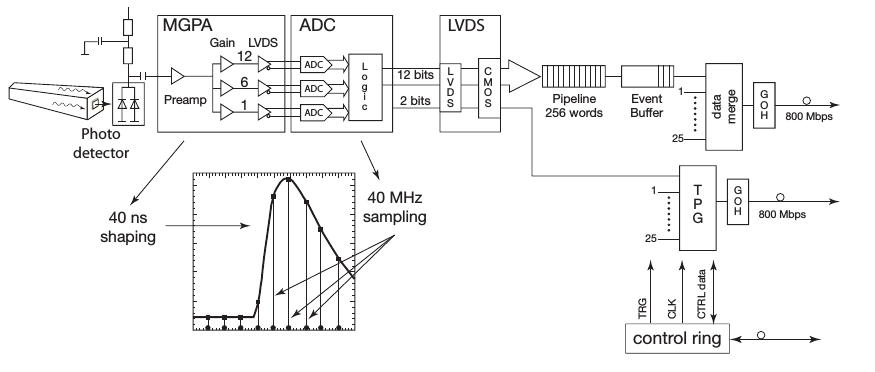
\includegraphics[height=0.5\textwidth, width=0.450\textwidth]{THESISPLOTS/ReadOut.png}
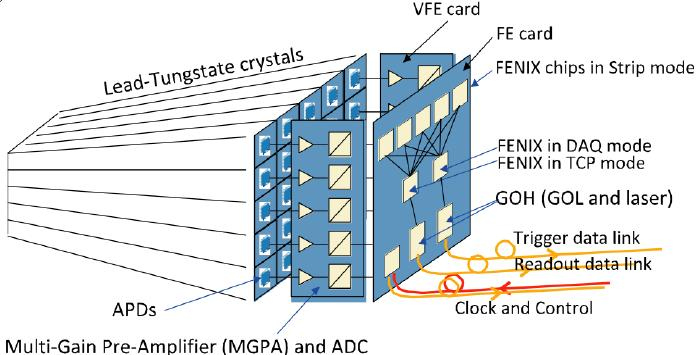
\includegraphics[height=0.5\textwidth, width=0.50\textwidth]{THESISPLOTS/ECAL-FRONT-END-ELECTRONICS.jpg}
%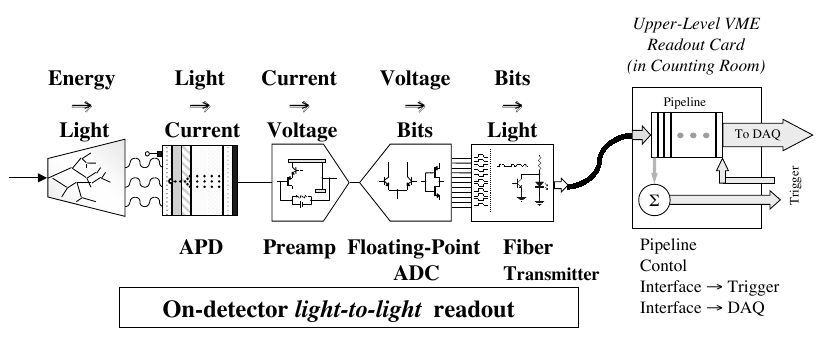
\includegraphics[height=0.5\textwidth, width=0.50\textwidth]{THESISPLOTS/CMS-ECAL-READOUT-CHAIN.png} \quad
} 
\captionof{figure}{Schematic diagram of the CMS ECAL electronics readout for a single channel(Left) and the entire Trigger Tower or Front End~(FE) Card(Right).}
\label{fig:readout}
\end{center}
 %%%%%%%%%%%%%%%%%%%%%%%%%%%%%%%%%%%%%%%%%%%%%%%%%%%%%%%%%%%%%%%%%%%%%%%%%%%%%%%%
\section{Time Reconstruction}\label{timereco}
%%%%%%%%%%%%%%%%%%%%%%%%%%%%%%%%%%%%%%%%%%%%%%%%%%%%%%%%%%%%%%%%
%Anlog signals from the APD/VPT of a single crystal is preamplified producing a typical signal pulse shown in figure \ref{fig:pulse}. 
An analog pulse shape from a single channel is shown in Figure \ref{fig:amplVsTmax}(a). 
Overlaying the pulse shape are typical 10 digitized  samples in red. The first three samples are taken in the absence of a signal and correspond to the pedestal.
The ADC chip responsible for the digitization, has a sampling frequency of 40~MHz, \ie one sample is made every 25~ns, which is the same rate as the LHC proton-proton bunch collision frequency of one bunch crossing every 25~ns.
In addition, the timing phase between each sample and the next is adjusted so that the maximum of the signal pulse shape corresponds to one of the samplings within 1~ns.
A time reconstruction algorithm uses these 10 digitized samples to measure the time of a single channel by finding the precise time corresponding to the maximum of the pulse shape, $\mathbf{T_{max}}$. 
% To measure the time, $\mathbf{T_{max}}$, corresponding to the maximum of the pulse shape,$\mathbf{A_{max}}$, a time reconstruction algorithm is used.

\begin{center}
\centering
\mbox{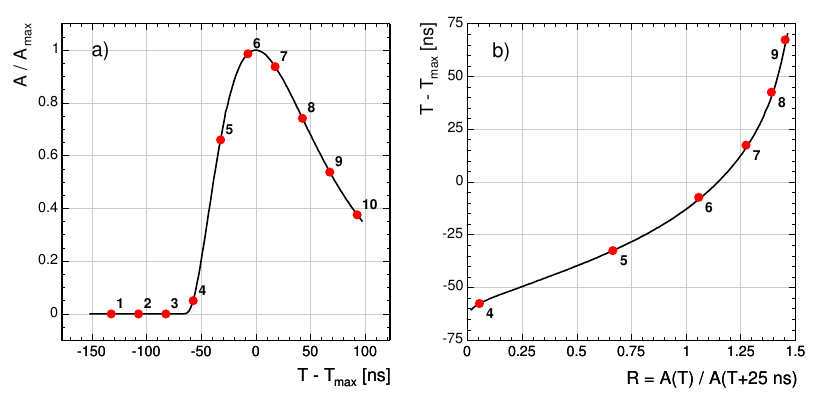
\includegraphics[height=0.50\textwidth, width=0.90\textwidth]{THESISPLOTS/AmplitudeVsTMax.png}}
%%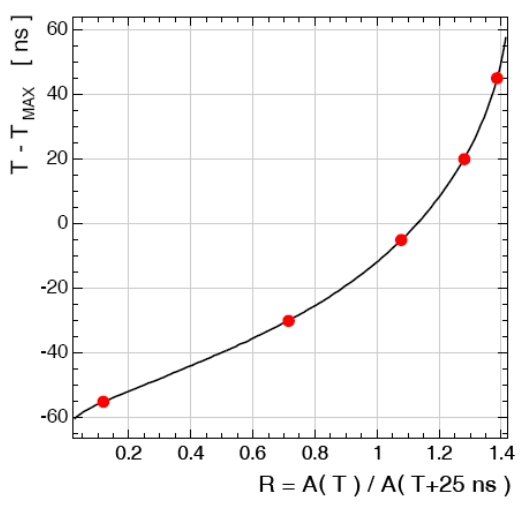
\includegraphics[height=0.45\textwidth, width=0.45\textwidth]{THESISPLOTS/TMaxPhaseVsRatio.png}}
%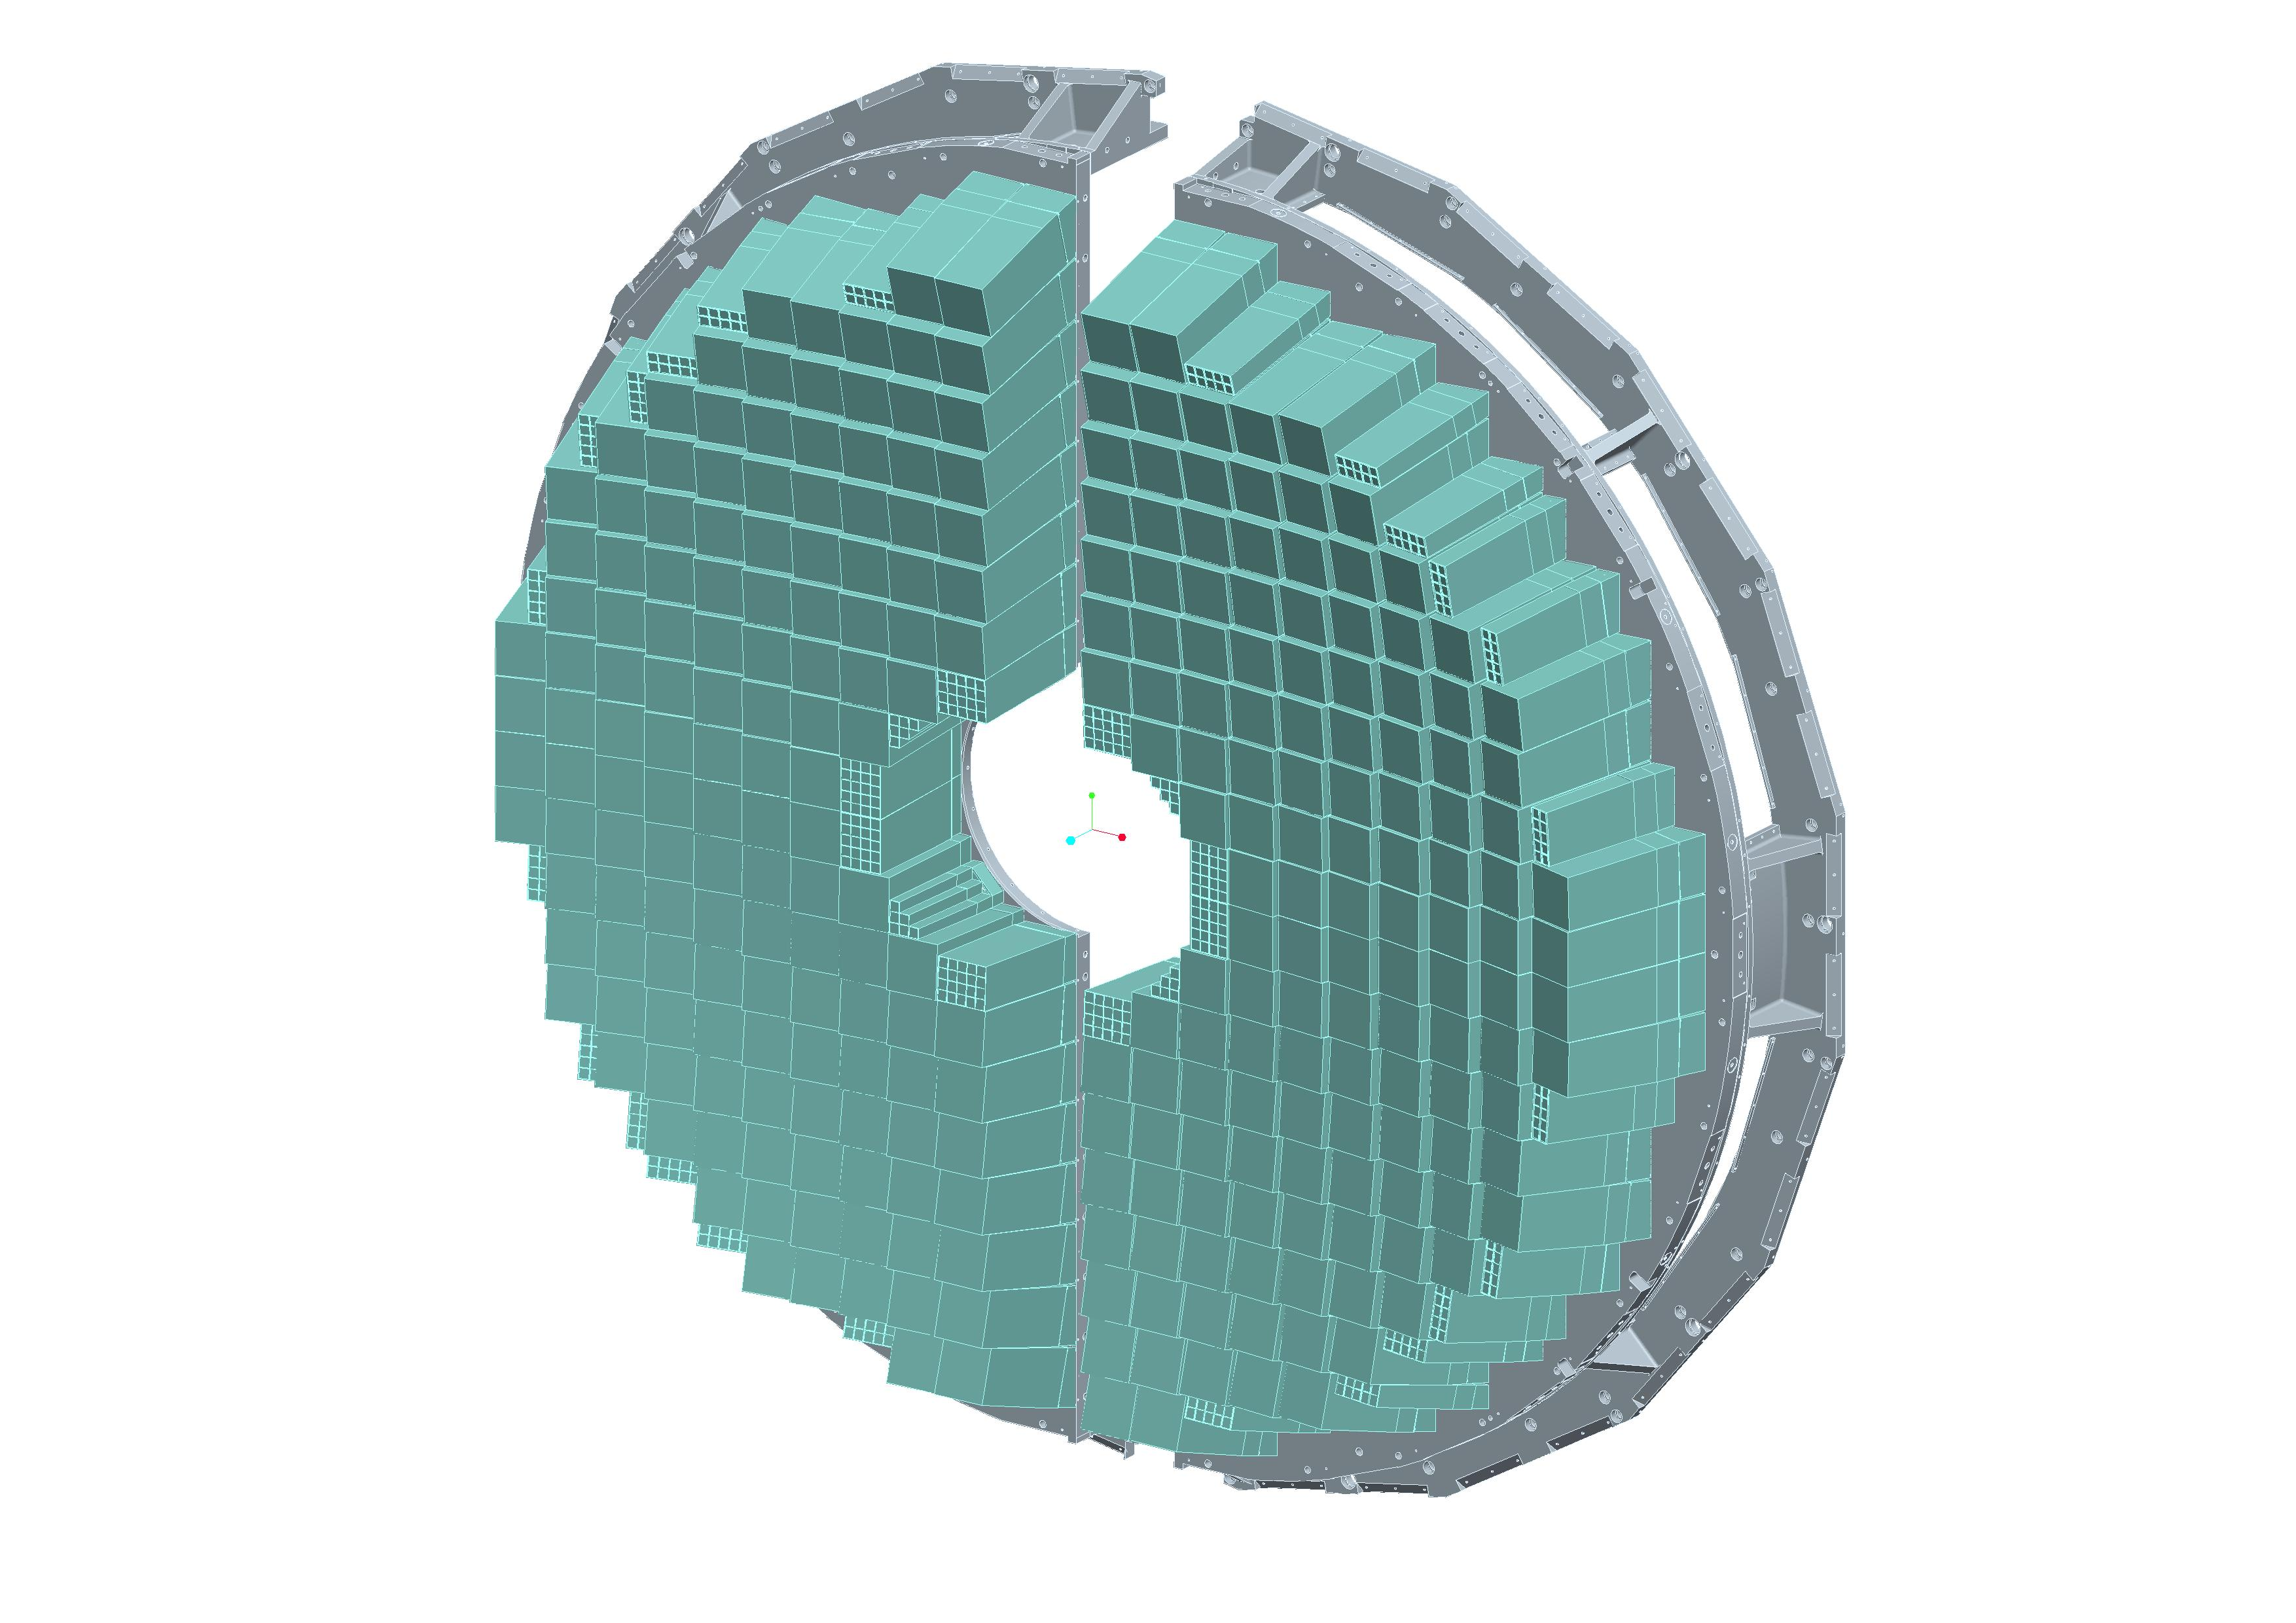
\includegraphics[scale=0.06]{THESISPLOTS/endcap_CMS.png}} 
\captionof{figure}{(a) A measured ECAL pulse shape for a single channel. (b) $\mathbf{T-T_{max}}$ Vs $ R(T)$ relationship whose inverse is $T(R)$. Solid line is pulse shape from test beam while dots are typical 10 discrete samples corresponding to signal from proton-proton collision.}
\label{fig:amplVsTmax}
\end{center}


\par
  Precise measurement of $\mathbf{T_{max}}$ relies on good knowledge of the pulse shape. To find $\mathbf{T_{max}}$ using the pulse shape, a ratio algorithm uses the ratio  
\begin{equation}{\label{eq:TREC}}
   R_{i} = A(T_{i})/A(T_{i+1}),
\end{equation}  
where $T_{i}$ is the time of the time of the beam crossing that the $i^{th}$ pulse height sample is taken. Each pulse height ratio is uniquely determined from the pulse shape as shown in Figure \ref{fig:amplVsTmax}(b) which shows the the pulse height ratio,$R_{i}$, as a function of the time that the pulse height of the first of a pair of samples is taken relative to the time of the maximum height of the pulse, $\mathbf{T_{i}-T_{max}}$. Using the inverse of this function, $T(R)$, we can obtained $\mathbf{T_{max}} = T_{i} - T(R_{i})$ and the uncertainty, $\sigma_{i}$, for each $R_{i}$ point. 
 %%where $\mathbf{T}$ indicates the time of an arbitrary ADC sample, depends on $\mathbf{A_{max}}$, the relative position of $\mathbf{T_{max}}$ between the time samples and the pulse shape itself and this  makes the time algorithm less precise when extracting $\mathbf{T_{max}}$ in this representation~($A(T)$) of the pulse shape. As a result, another representation of the pulse shape measured a function of a ratio variable, $R(T) = A(T)/ A(T + 25~\mbox{ns})$, which is independent of $\mathbf{A_{max}}$, is rather used in the time algorithm. The representation of the pule shape as a function of $R(T)$ is shown in \ref{fig:amplVsTmax}(b) and can be  modeled easily with a simple polynomial function.The parameters of the polynomial were measured during electron test beam experiments by fitting to the pulse shape of the test beam data.% can be used to model the pulse shape as a function of $R(T)$ favors using the pulse shape as a function of $R(T)$ in the time extraction algorithm. %where the distribution of $T - \mathbf{T_{MAX}}$ as a function of $ R(T)$ is presented. This representation can easily be well described using a polynomial function.
%Extracting of the arrival time is by comparing the pulse shape of a channel obtained during proton-proton collision to a reference pulse shape obtained during early LHC \textit{test beam} results.
%This reference pulse shape has been obtained from  measurements using synchronous LHC events. Figure \ref{fig:amplVsTmax}(\textit{Left}) shows a distribution of $A/\mathbf{A_{MAX}}$ on the vertical axis against $T - \mathbf{T_{MAX}}$ on the horizontal axis obtained from test beam experiments. $T$ is an arbitrary time  measurement and $\mathbf{T_{MAX}}$ is the time when the  pulse reaches its maximum value, $\mathbf{A_{MAX}}$.
%%\begin{center}
%%\centering
%%\mbox{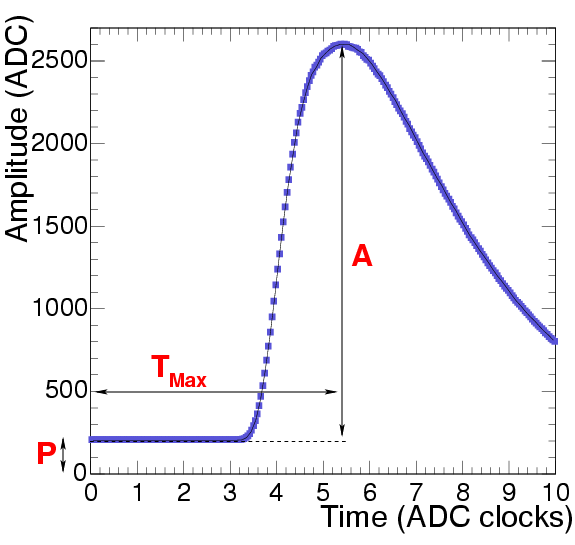
\includegraphics[height=0.5\textwidth, width=0.5\textwidth]{THESISPLOTS/Time_Amplitude_Profile.png}}
%\mbox{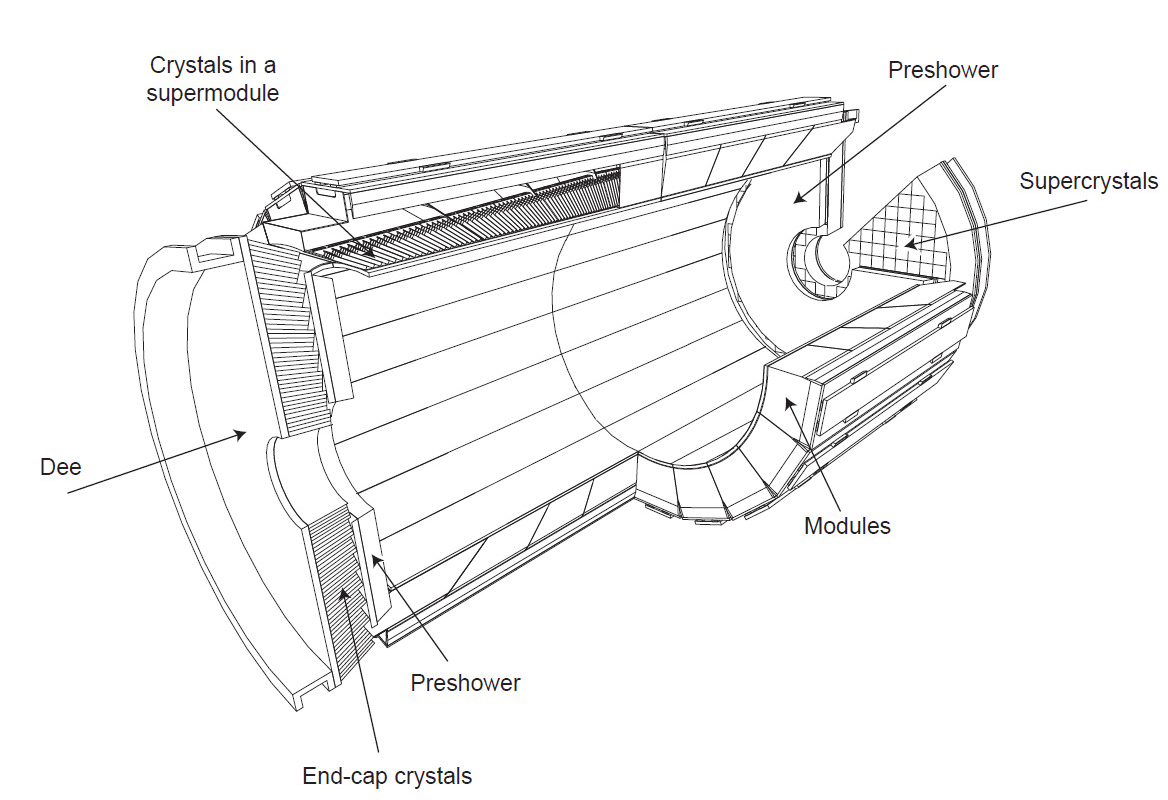
\includegraphics[scale=0.2]{THESISPLOTS/CMS-ECAL.png}}
%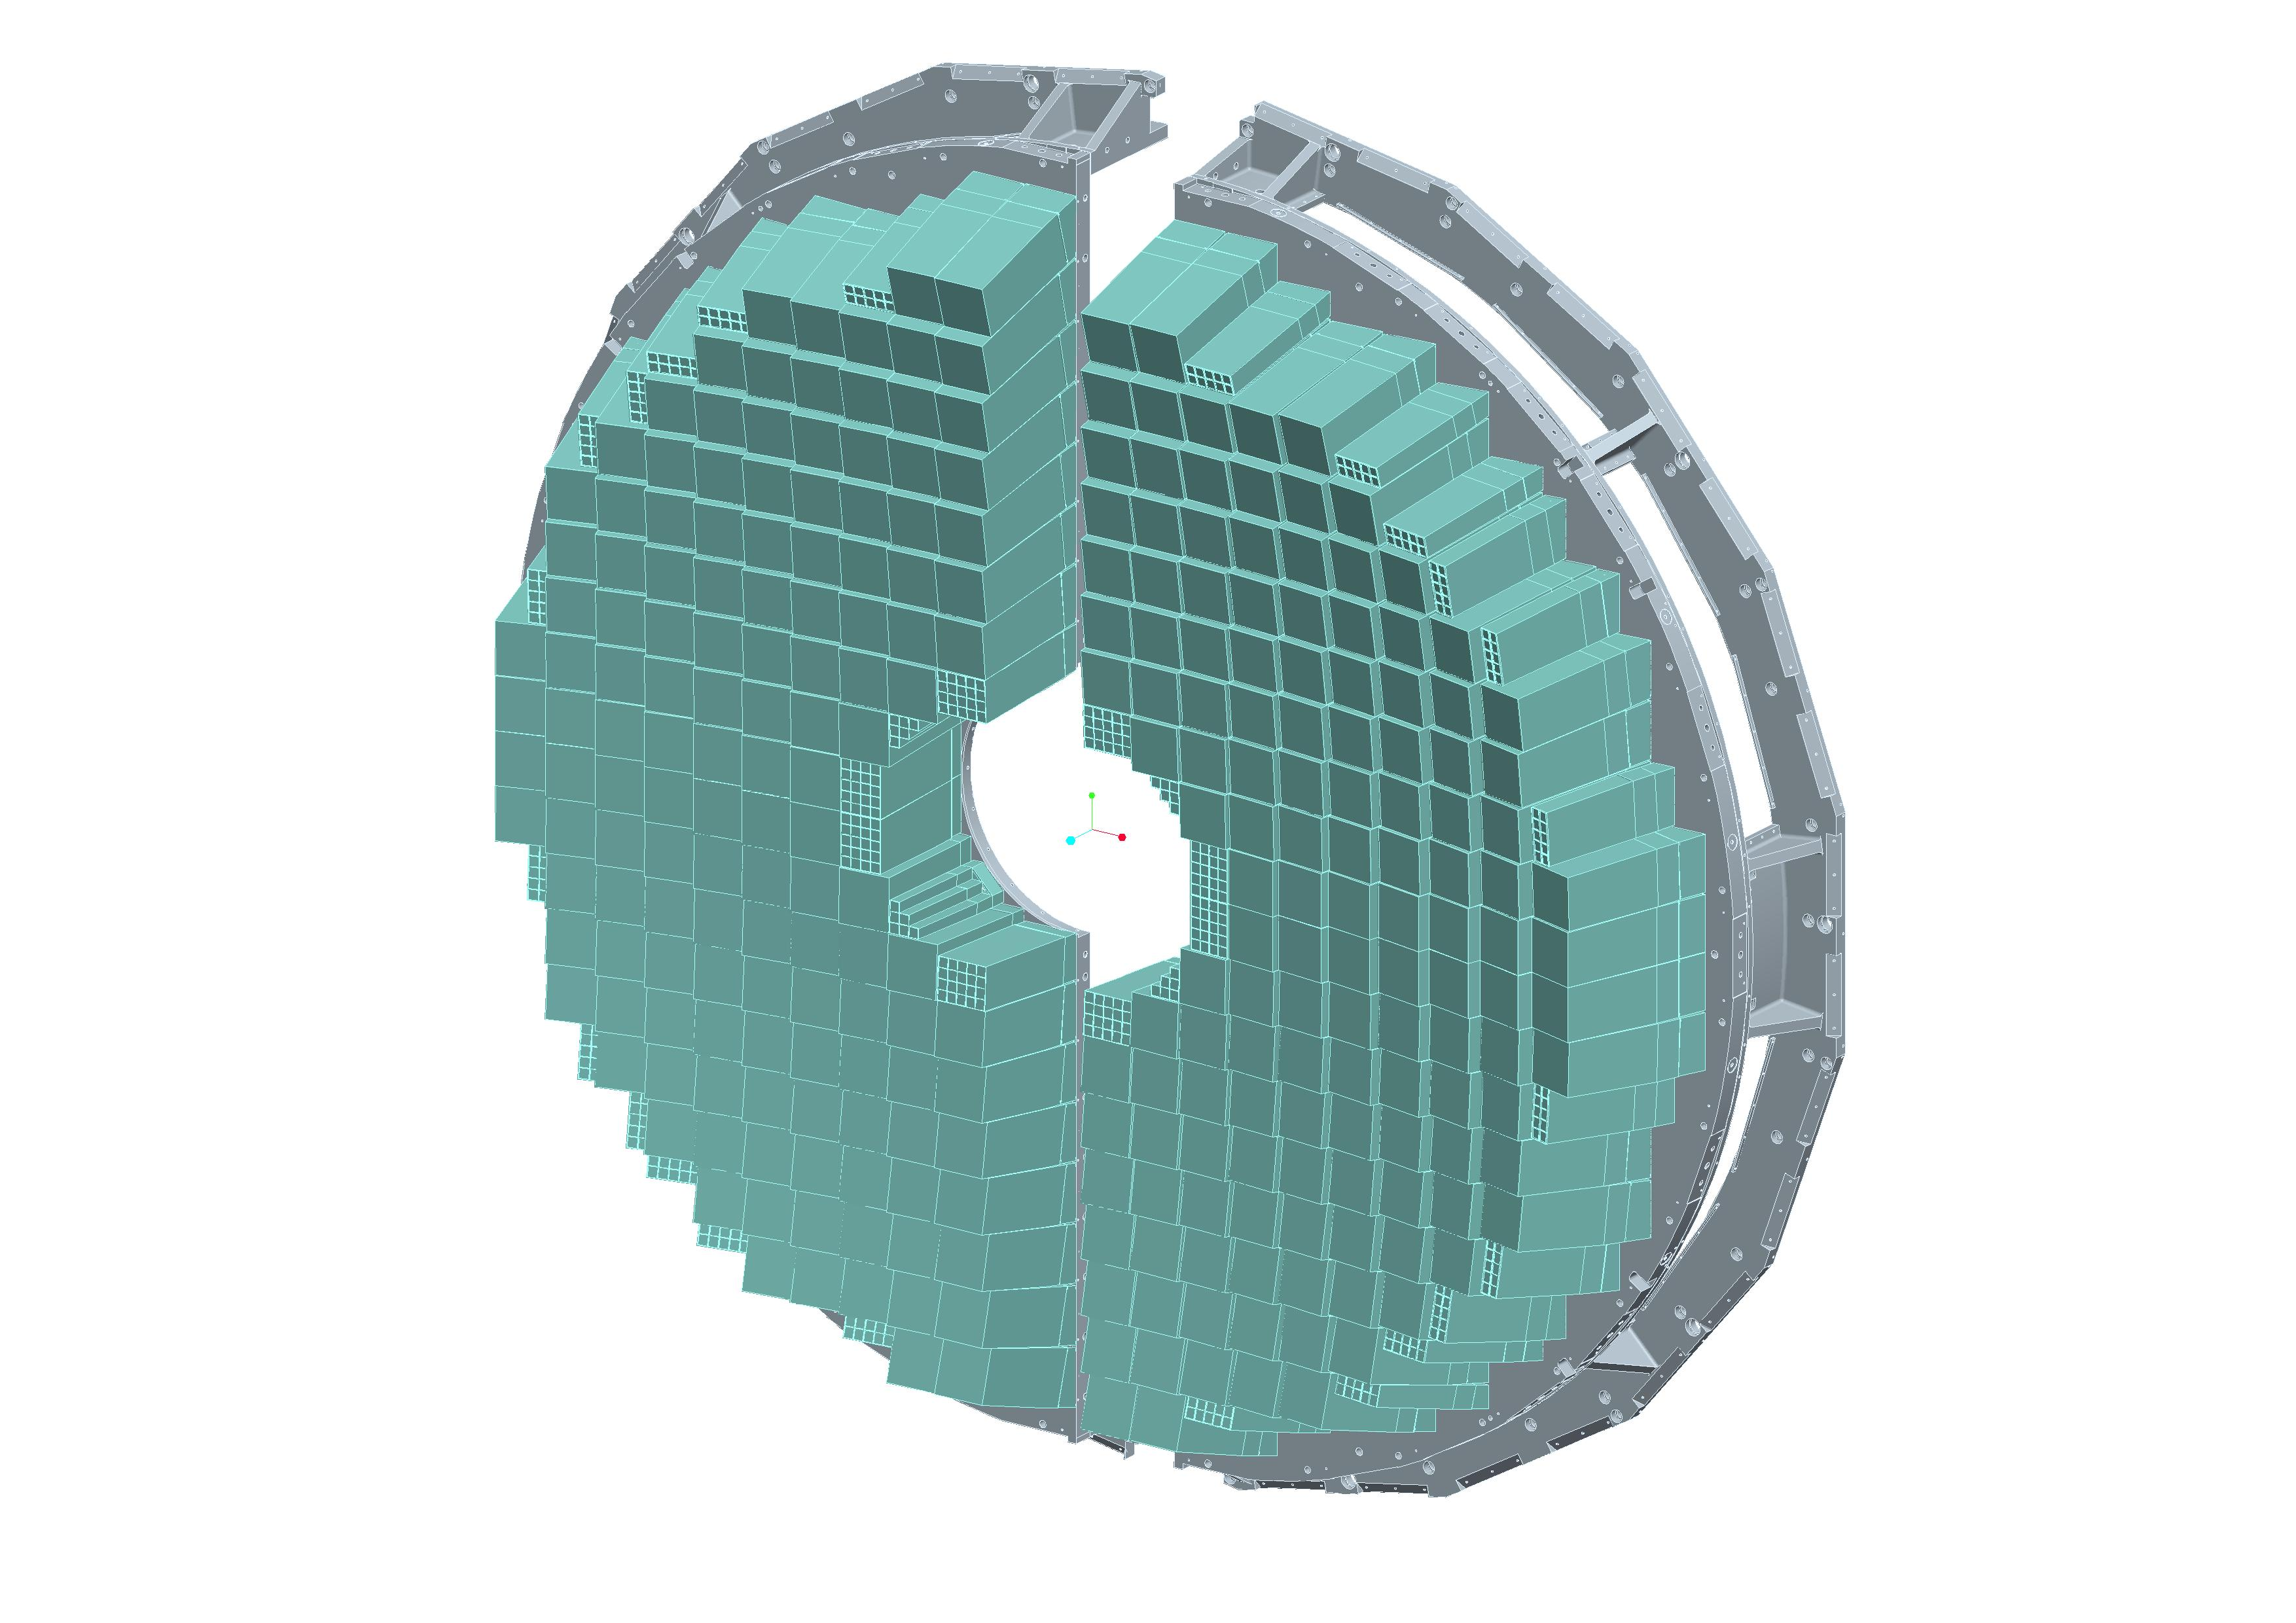
\includegraphics[scale=0.06]{THESISPLOTS/endcap_CMS.png}} 
%%\captionof{figure}{Typical pulse shape of a given signal showing crystal signal.}
%%\label{fig:pulse}
%%\end{center}
%\par
%This representation~($T(R)$) of the pulse shape as a function of $ R(T)$, usually consist of 5 or 6 sample points~(dots) obtained from the ratio of consecutive pair of samples, $R_{i} = A(T + i\cdot25~ns)/A(T + (i+1)\cdot25~ns)$, of a typical reference pulse shape~(continuous line). 
%From each $R_{i}$ point we obtain a quick accurate measurement of $T_{max,i} = T_{i} - T(R_{i})$ and the uncertainty, $\sigma_{i}$. 
\newline
The uncertainty on each measurement is a product of the derivative of the function $T(R)$ and the uncertainty on the value of $R_{i}$ which itself depends on three separate uncertainties: the noise fluctuation~($\sigma_{n}$) of each sample, the uncertainty in the estimation of the pedestal value which is always subtracted from the measured value and the truncation during 12-bit digitization. These uncertainties are uncorrelated and can be added in quadrature,\cite{TIME}.
\newline
A more precise value of $T_{max}$ is obtained by using the ratios $R_{4}$ through $R_{7}$. The other ratios are not used  for the estimation of $T_{max}$ because their associated uncertainties are large due to the large slope of the $T(R)$ function.  A weighted average of each $T_{max}$ and $\sigma$ obtained from ratios $R_{4}$ through $R_{7}$ as expressed in Equation \ref{eq:TMAX} gives the best estimate of $T_{max}$ and uncertainty.
\begin{equation}{\label{eq:TMAX}}
\displaystyle{T_{max} = \frac{\sum \frac{T_{max,i}}{\sigma^{2}_{i}}}{\sum \frac{1}{\sigma^{2}_{i}}}} \quad , \quad\quad
\displaystyle{\frac{1}{\sigma^{2}_{T}} =  \sum \frac{1}{\sigma^{2}_{i}} }
\end{equation}
The sum is from  $i = 4,\cdots,7$.% and the assumption is that the weights are uncorrelated. % These parameters obtained are subsequently use by the ECAL time algorithm to reconstruct time during proton-proton collisions.

%%%%%%%%%%%%%%%%%%%%%%%%%%%%%%%%%%%%%%%%%%%%%%%%%%%%%%%%%%%
\section{ECAL Time Performance from Test Beam}
%%%%%%%%%%%%%%%%%%%%%%%%%%%%%%%%%%%%%%%%%%%%%%%%%%%%%%%%%%%
%%The energy recorded by each crystal is called a \textit{hit}.  Using this hit, we can calibrate the time of each of the  75,848 ECAL crystals to ensure that the arrival time of an electromagnetic particle of an event is accurately measured.
%To be able to precisely measure the arrival time, the crystals must be well calibrated. 
%%Crystal time calibration means defining the same reference time used by each crystal for measuring
%%the particle's arrival time. This can be achieved by using an electromagnetic particle like a photon, produced from a $pp$ collision
%%at IP, and whose trajectory or path traveled from IP to the surface of a crystal and traveling with the speed of light 
%%is a straight line. For such a particle, its time-of-flight~(TOF) is the ratio of the distance traveled to the speed of light.
%%The photon time measured by each ECAL crystal is assumed to be the same for every other crystal and defines the absolute or reference time for every other similar electromagnetic particles. The time needed to transfer the recorded signal from the front-end detectors to the back end readout electronics is also assumed to be the same for all crystals. Taking the TOF into account, we define the crystal time, $\left\langle t \right\rangle \approx 0$ as the reference time for the time measurement of the photon by each crystal.
%%Thus, if a crystal is properly calibrated, then the average time for hits belonging to the same event
%%must be zero, \ie, $\left\langle t \right\rangle_{\mbox{many hits}} \approx 0$. 
\subsection{ECAL Time Resolution}
The intrinsic time resolution of ECAL, $\sigma(t)$, measured during test beam, consist of three main contributions which can be summed in quadrature since they are uncorrelated. These three contributions are the noise, stochastic and constant terms. The \textit{Noise}~($N$) term arises from the electronic noise, coherent movement of the baseline and effects overlapping hits some of which come from other soft proton-proton collisions called \textit{pile up}~(PU) events. The \textit{Stochastic} term~($S$) is from fluctuations in the number of photons collected during the sample times. Lastly, the \textit{Constant} term~($C$), whose contribution is independent of the energy deposited and arises from variations in the point of shower initiation within the crystal and variations in the pulse shape for each channel.
The full expression for time resolution with all three contributions is given in Equation \ref{eq:TimeRes},

\begin{equation}{\label{eq:TimeRes}}
\sigma^{2}(t) = \left(\frac{N}{A/ \sigma_{n}}\right)^{2} + \left(\frac{S}{\sqrt{A}}\right)^{2} + C^{2},
\end{equation}
where $A$ is the measured amplitude corresponding to the energy deposited and $\sigma_{n}$ is the intrinsic noise in the amplitude for individual channel. $\sigma_{n}$ has a value of $42$~MeV and $140$~MeV in the barrel and endcap, respectively. $N = 33$~ns has been estimated from Monte Carlo~(MC) simulation studies. Contribution from the stochastic term, ($S$) is small, with a value of $S < 7.9$~ns$\cdot MeV^{1/2}$.
\par
    To measure the intrinsic time resolution of ECAL and study the pulse shape, H2 and H4 test beam facilities at CERN were used.
Prior to installation at the CMS detector, about 25\% of the barrel and endcap crystals were exposed to electron beams with energy  between 15\GeV and 250\GeV. The time resolution was obtained from the Gaussian distribution of the difference in time of two crystals sharing energy and belonging to the same electromagnetic shower. Note that the contribution from crystal-to-crystal synchronization  does not contribute to the constant term in this study. Neglecting the stochastic term because its contribution is negligible, Equation \ref{eq:TimeRes} reduces to:
\begin{equation}{\label{eq:TIMERES}}
 \sigma^{2}(t_{1} - t_{2}) = \left(\frac{N}{A_{eff}/ \sigma_{n}}\right)^{2} + 2\bar{C}^{2}
 \end{equation}
where $A_{eff} = A_{1}A_{2}/\sqrt{A^{2}_{1} + A^{2}_{2}}$, while $t_{1,2}$ and $A_{1,2}$ are the times and amplitudes of the two crystals. $\bar{C}$ is their residual constant term contribution. 
The time resolution is measured from the standard deviation of a Gaussian fit to the time distribution from each slice of $A_{eff}/\sigma_{n}$ of the $A_{eff}/\sigma_{n}$ distribution. The resulting distribution of $\sigma(t_{1} - t_{2})$  of these standard deviations plotted against $A_{eff}/\sigma_{n}$ is used to extract the noise and residual constant terms.  The result presented in Figure \ref{fig:FitTimeRes} gives a noise factor $N = (35.1 \pm 0.2)$~ns and $\bar{C} = (20 \pm 4)$ ~ns  obtained from test beam experiment. 
\newline 
The value of the $N$ in this study agrees with our Monte Carlo estimate to within 6\%.
% It is this approach which we employ in future studies of the ECAL timing resolution.
\newline
Other studies of the timing resolutions using the time difference between two basic clusters of separate electromagnetic shower was used and the results gave similar values of $N$.
\begin{center}
\centering
\mbox{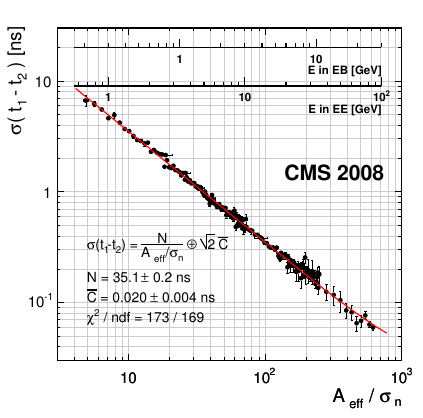
\includegraphics[height=0.60\textwidth, width=0.85\textwidth]{THESISPLOTS/ECAL_Timing_Resolution.png}}
%\mbox{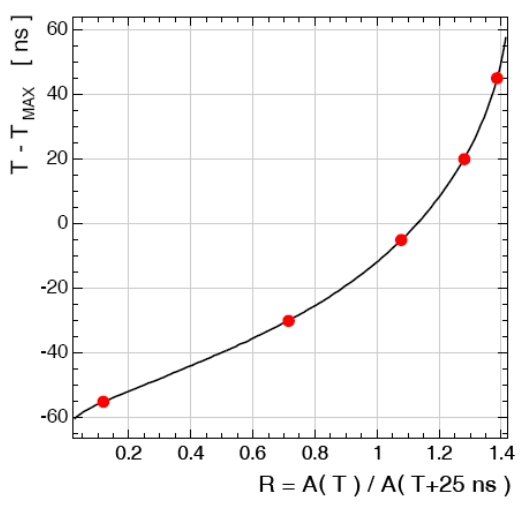
\includegraphics[scale=0.45]{THESISPLOTS/TMaxPhaseVsRatio.png}}
%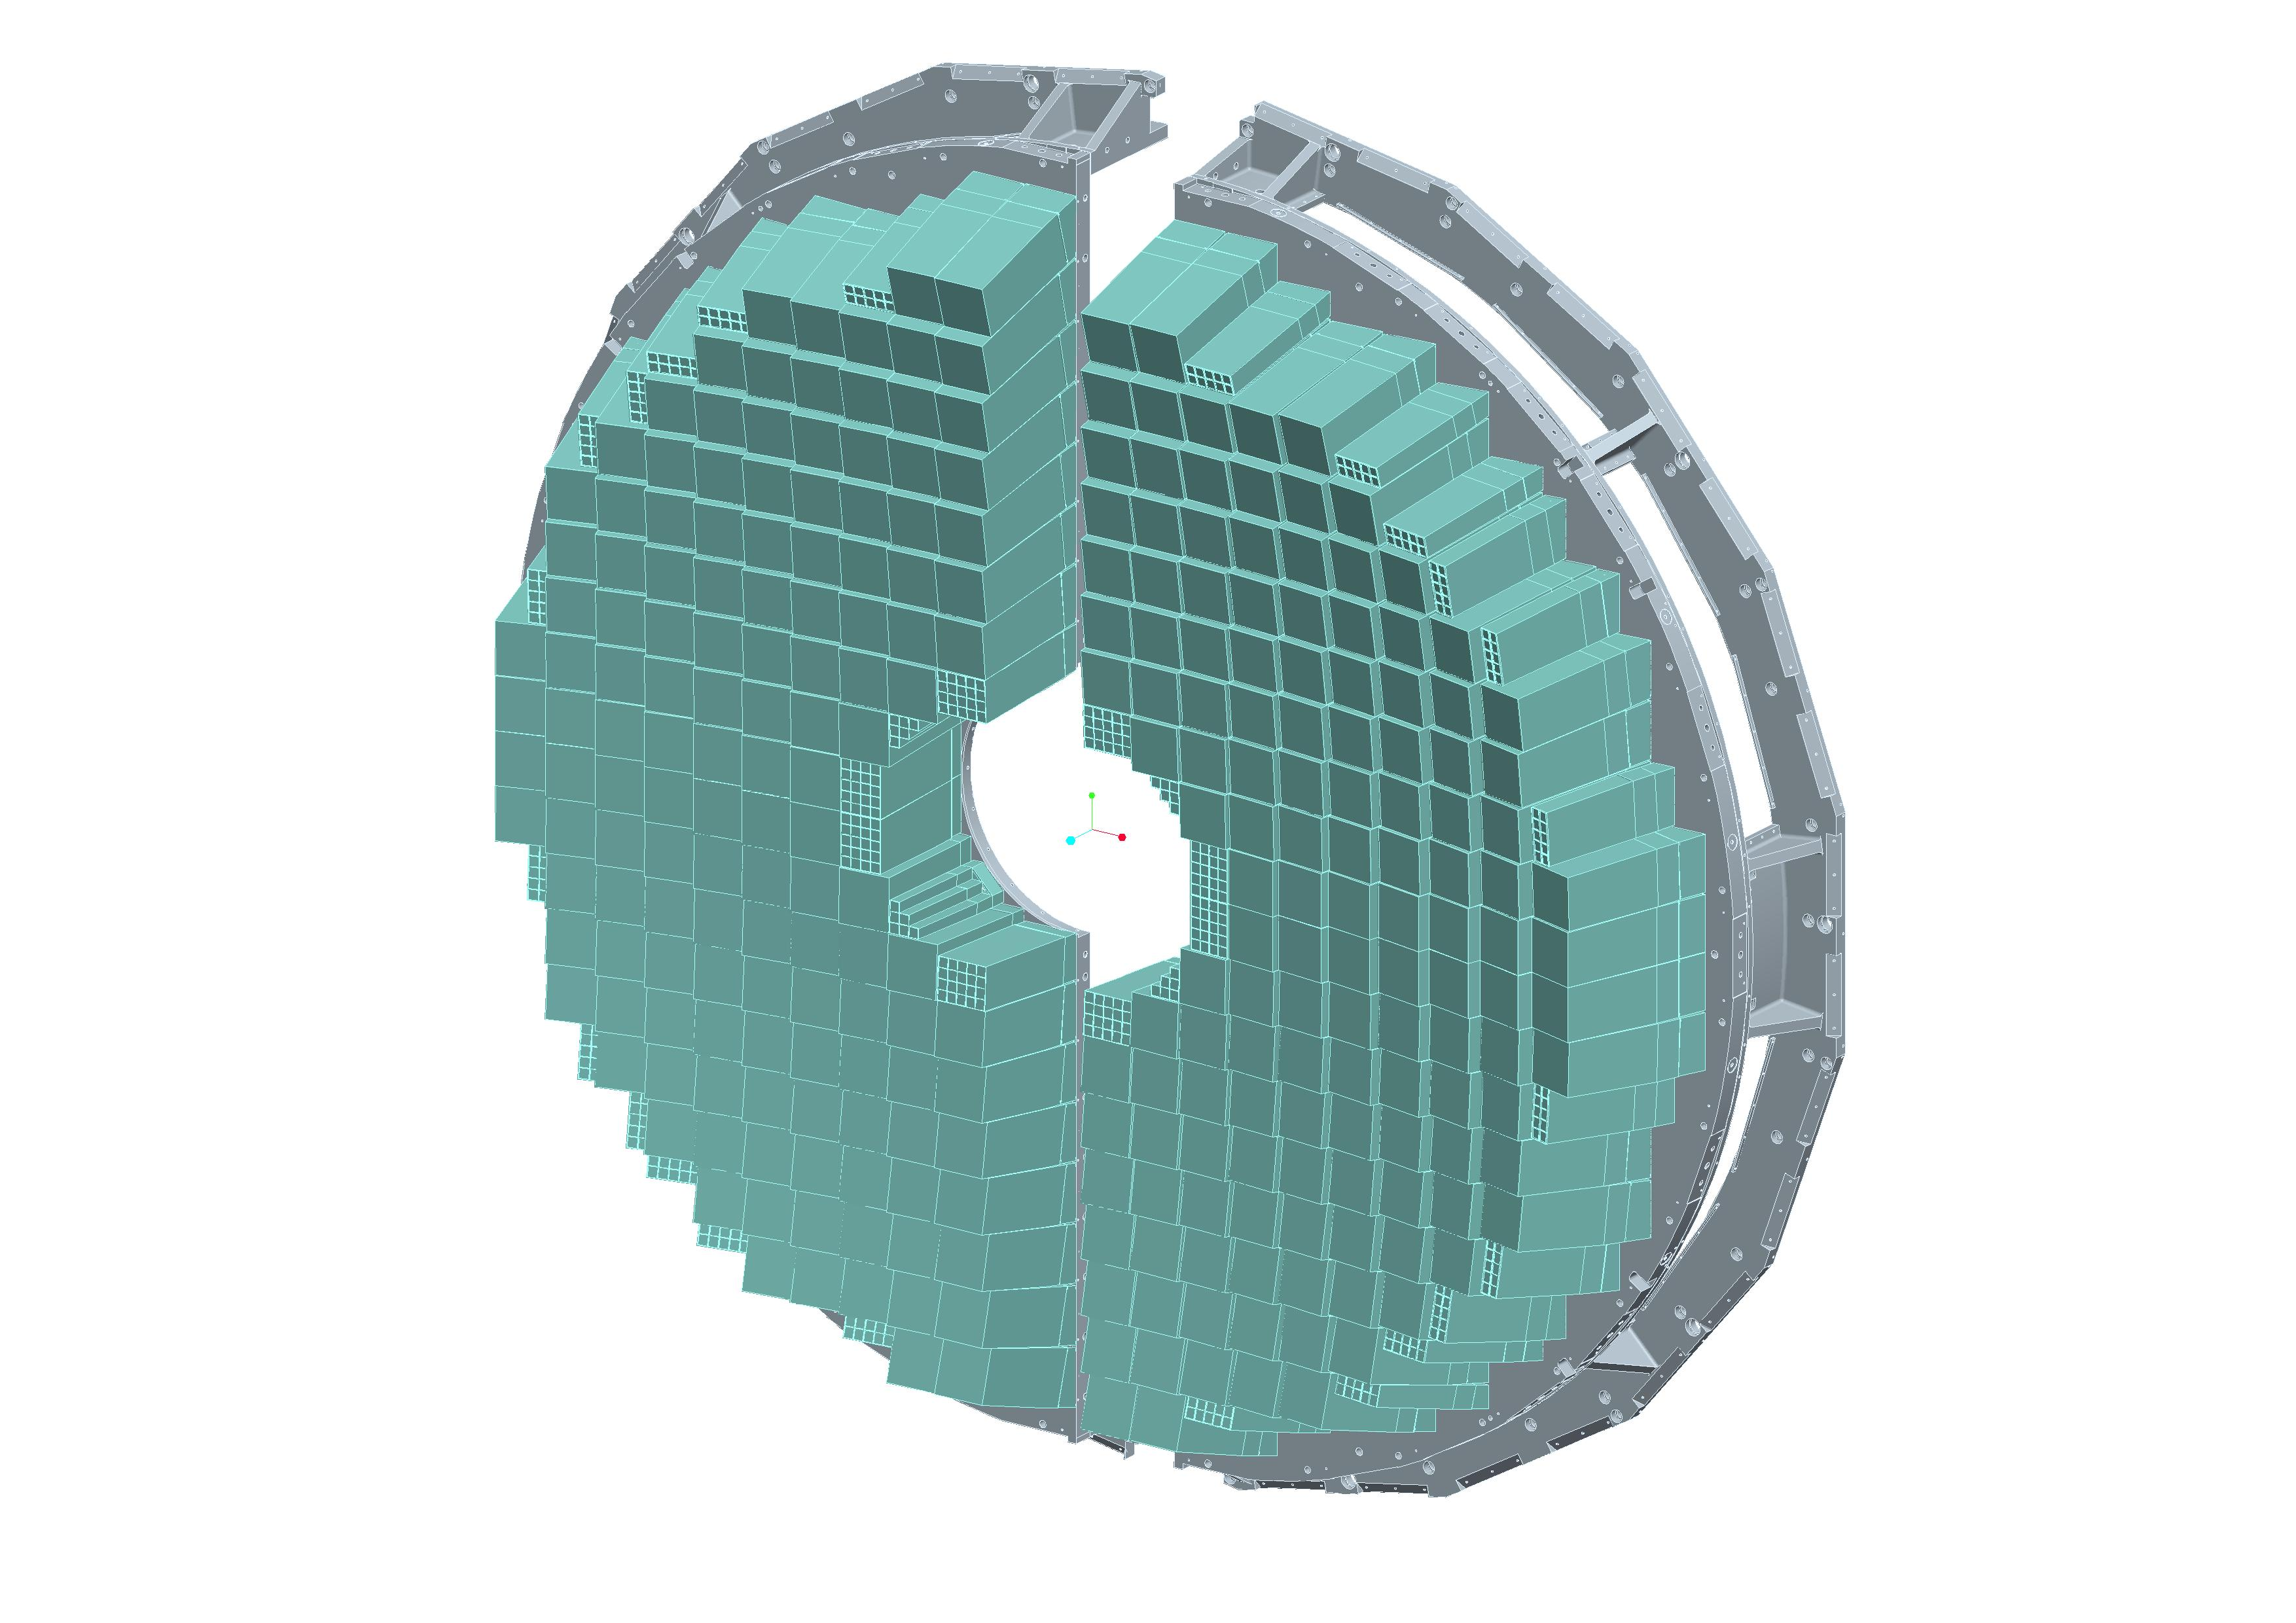
\includegraphics[scale=0.06]{THESISPLOTS/endcap_CMS.png}} 
\captionof{figure}{Difference in the time measurements as a function of $A_{eff}/\sigma_{n}$ of two crystals sharing an energy and belonging to the same electromagnetic shower obtained during electron testbeam measurements. The single crystal energy scales for barrel~(EB) and endcap~(EE) is overlaid. The fitted results give $N = (35.1 \pm 0.2)$~ns and $\bar{C} = (20 \pm 4)$ ~ns. }
\label{fig:FitTimeRes}
\end{center}
\paragraph{} %% Need for Timing resolution from collision
An intrinsic time resolution  better than $0.1$~ns for energy $E > 20$\GeV in EB is realized from test beam. Knowing that it takes on average 4.3~ns for a photon to reach the ECAL surface produced from proton-proton interaction point, this demonstrates an intrinsic time resolution of 2\% for photons with energy $E > 20$~GeV in the barrel.%, a time resolution better than 100~ps can be realized during proton-proton collisions. %we can obtain a resolution better than $100$~ps. 

%%%%%%%%%%%%%%%%%%%%%%%%%%%%%%%%%%%%%%%%%%%%%%%%%
\section{ECAL Time Performance from Collision}
%%%%%%%%%%%%%%%%%%%%%%%%%%%%%%%%%%%%%%%%%%%%%%%%%%%%%
Ofcourse, we do not expect the ECAL time resolution in the LHC proton-proton collision environment to be as precised as test beams studies show. Therefore, it is imperative to determine the ECAL time resolution in an LHC environment as knowing the ECAL time resolution in LHC operation can be used for other purposes like eliminating particles such as cosmic rays, beam halo muons, electronic noise and out-of-time proton-proton interactions with broad time distributions. There are factors like clock time variations over extended time, timing bias with energy and looses in crystal transparency due to radiation which would lead to different pulse shapes which worsen the ECAL time resolution. Thus, a robust crystal time calibration procedure is required if we are to match the intrinsic time resolution realized in test beam studies that we mentioned above. In addition, precise ECAL time during collision can be use in the search for photons with late arrival time produced from the decay of slow moving particles with $\beta << 1$, photons traveling along a path which significantly deviates from the obvious straight path from the proton interaction point.% indicating the presence of a highly boosted particle or could be photons and electrons produced in the decay of a temporarily stopped particle inside the CMS detector.
\subsection{Time Calibrations}
%%%%%%%%%%%%%%%%%%%%%%%%%%%%%%%%%%%%%%%%%%%%%%%%%%%%%%%%%%%%%%%%%%
Variations in the crystal time maybe caused by the non-uniform response to electromagnetic showers of each crystal causing difference in pulse shapes or by clock time shifts introduced by interventions during technical shutdowns for machine repairs. These variations can be about 1 to 3 ns on average. To reduce these contributions, we continuously time align all 75,848 \pb crystals in ECAL by performing crystal \textit{time calibration} once or twice every month. 
Time calibrating these crystals ensures that there is a uniform response by all the crystals to photons produced from proton-proton collisions, at interaction point, and traveling along a straight path with speeds close to the speed of light to ECAL. It equally guarantees the synchronization of most particles of an event and assigns each event to the correct LHC proton bunch crossing. 
\newline
The presence of the "$T_{max}$ Phase", the difference in pulse shape between each crystal, variation in time of flight by a few nanosecond~(ns) and the different intrinsic delays in each channel motivates a time calibration at two separate levels. At the level of the front end electronics ~(FE) consisting of $5\times5$ crystals, We perform an initial internal time synchronization by adjusting the time measured by each trigger tower in steps of 1.04~ns among all the trigger towers. Determining the trigger tower time constants needed for time aligning these trigger towers takes place during the process of \textit{Hardware Synchronization}. Offline, we assign time constants to each crystal, during hit reconstruction using the CMS reconstruction software during the transition from uncalibrated hits to calibrated hits.
%such that the time of flight for photons traveling along a straight path directly from the proton-proton interaction point to the crystals is the absolute measured time by all the crystals.
%The time adjustments constants are developed separately for the barrel and endcaps.
%There are significant benefits to having a uniform time alignment by all the crystals. With a better time calibrated detector, it is possible to distinguished between photons or electrons with significantly large arrival time from normal in-time photons produced in collisions. 
 

\subsubsection{Offline Time Calibration}
The purpose of the offline calibration is to provide time calibration constants for each crystal during event reconstruction. These constants are derived from data recorded during  proton-proton collisions and are used to adjust for any clock time shift. A crystal time shift of about 1~ns is caused by the relative time shift between the CMS and the LHC clocks and time shift of about 3~ns to 5~ns is caused by time offsets in the local CMS clock introduced during hardware interventions. The local time offsets is specific only to certain regions of the ECAL detector.
The calibration constants for each crystal is the reverse sign of the average time of all the reconstructed energy deposits~(rechits) in the crystal.
New sets of calibration constants are produced each month throughout the entire LHC run period.
Each set of time constants produced has an \textit{interval of validity}~(IOV).
A total of 17 IOV time constants were produced for the entire LHC run in 2011 and 44 IOV time constants for 2012.
%The calibration procedure begins with identifying  timing shift reported in the CMS or ECAL detector running electronic~(e-Log) book or the CMS or ECAL data acquisition monitoring~(DQM) and followed by using  reconstructed crystal hits or rechits from recently recorded or prompt data to measure the calibration constants for each channel. The validated calibration constants in an XML files are uploaded into the online configuration database with existing hardware settings for reprocessing of CMS full datasets used for physics analysis.
%This process is performed throughout the entire LHC proton-proton collision period each year. At the end of each calibration process, the set of calibration constants developed for that period of time is called its . The data used in measuring the timing constants is specified by run range of events signifying a period over which proton-proton collisions occurred. During the entire LHC run period in 2011, a total of 17 IOVs were developed while during 2012 LHC run, a total of 44 IOVs were produced. The raw dataset used in producing the calibration constants consists of mostly superclusters with crystal hits from Level-1 triggered events of loosely triggered  photons, electrons and hadrons with large electromagnetic contributions. Datasets with such events are called \textit{ElectronHad} or \textit{PhotonHad}. Rechits from these events must pass a selection criteria which include, the event time~(an average over it's rechits) must be smaller than 5~ns, rechits must belong to a basic cluster whose transverse energy is atleast 2~\GeV, the signal amplitude must not be lower than 26(47) or 100~(in LHC 2012) ADC counts~(corresponding to an energy of about 1(3)~GeV ) for rechits in EB(EE), the reconstructed rechit time must be within 5(7)~ns from either side of zero in EB(EE) and to reduce the presence of anomalous crystal hits, the ratio of the sum of energies of the north, south, east and west neighboring crystals excluding the crystal with the highest energy to that of the energy of the highest energy crystal must be greater than 5\%  or equivalently $ 1 - E_{4}/E_{1} < 0.95$~(the \textit{swiss-cross} variable). This swiss-cross variable is very useful for rejecting events with anomalous crystal energy deposits. The selected rechits are used to make a timing distribution for each channel requiring each channel to have at least 10 rechits.
%After extracting the average time per crystal, the reverse of its value measured is the time calibration constants or inter-calibration coefficient used for timing alignment. The variance represents the spread in the measurement of the calibration constant. For channels with less than 10 valid rechits, the average time of all the other channels is assigned to them as their inter-calibration coefficient. We validate these constants obtained by performing a closure test which involves  applying the reversed values of these constants to the same or different set of events and showing that the measured average time over rechits per channel is 0~ns to within the accuracy of the calibration method and small event migration in the event sample. The event migration effects are of the order of 10~ps.
\newline
The data sample use for producing the calibration time constants contains mostly electromagnetic particles of mostly loosely triggered photon, electron and hadrons with large electromagnetic shower which travel with nearly the speed of light and largely deposit  most of their energy at ECAL. Events of these data samples undergo a rigorous event selection process in order to minimize contamination from events not produced from proton-proton collisions like cosmic muons, beam halos and electronic noise. The produced constants are validated through a full cycle hit reconstruction-time adjustment-hit re-reconstruction procedure of a chosen sub data sample. The validate constants are then used during full event reconstruction.
The maps in Figure \ref{fig:TimeCalib}, show two dimensional distribution maps of the average time~(time calibration constants) for each of the 61,200 crystals in EB and 14648 crystals in EE. The figure shows each crystal average time before~(\textit{top 3 plots}) and after~(\textit{bottom 3 plots}) calibration. More information about crystal time calibration for the entire LHC Run 1 is found in \cite{ECALCAL}.
%%%%%%%%%%%%%%%%%%%%%%%%%%%%%%%%%%%%%%%%%%%%%%%%%%%%%%%%%%%%%%%%%
\begin{center}
\centering
\mbox{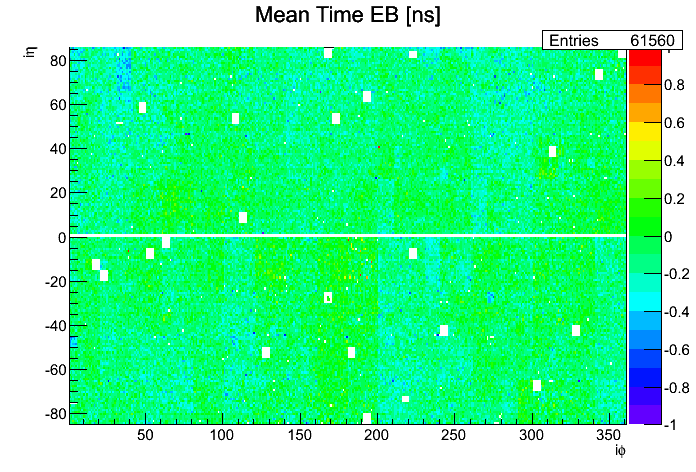
\includegraphics[height=0.50\textwidth, width=0.80\textwidth]{THESISPLOTS/calibDiffMapEB_Before_Calibration.png}}
\mbox{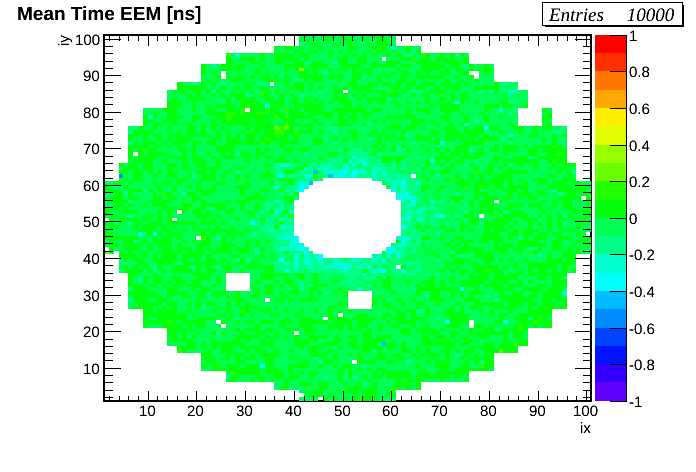
\includegraphics[height=0.52\textwidth, width=0.45\textwidth]{THESISPLOTS/calibDiffMapEEM_Before_CALIB.png} \quad
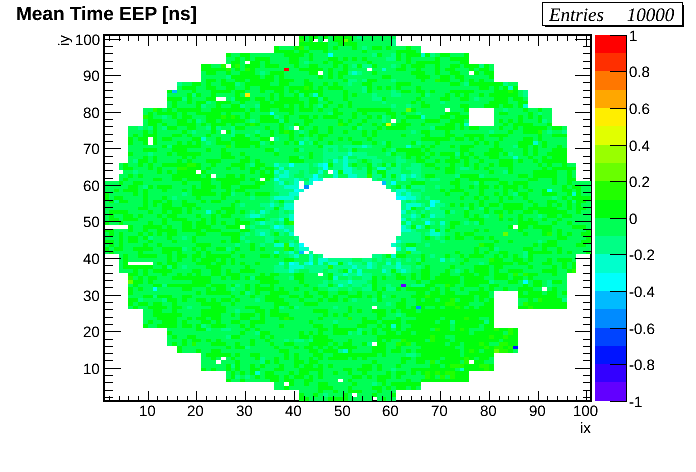
\includegraphics[height=0.52\textwidth, width=0.45\textwidth]{THESISPLOTS/calibDiffMapEEP_Before_CALIB.png}
}
%\hline
%\vspace{1.5cm}
\clearpage

\mbox{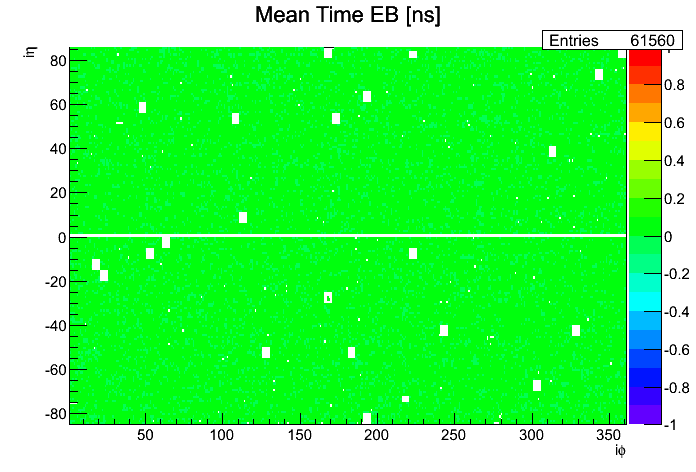
\includegraphics[height=0.50\textwidth, width=0.80\textwidth]{THESISPLOTS/calibDiffMapEB_After_Calibration.png}}
\mbox{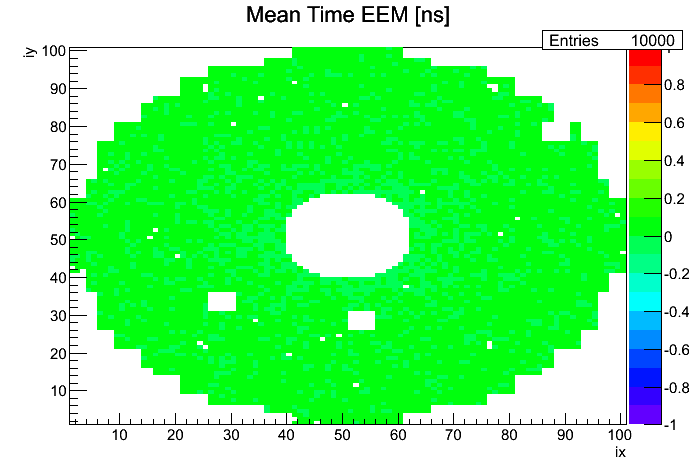
\includegraphics[height=0.52\textwidth, width=0.45\textwidth]{THESISPLOTS/calibDiffMapEEM_AFter_CALIB.png} \quad
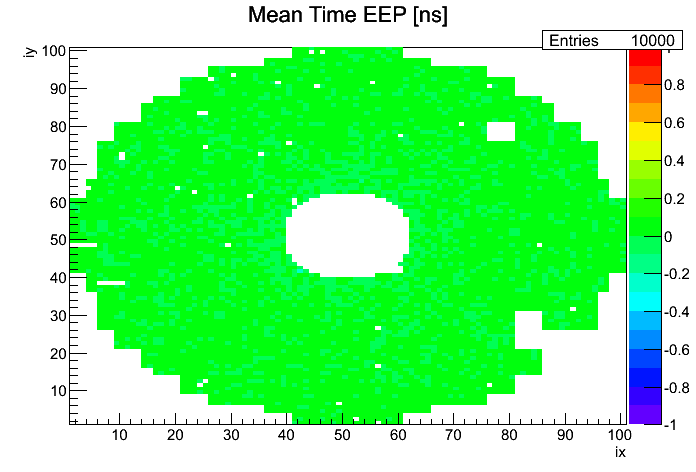
\includegraphics[height=0.52\textwidth, width=0.45\textwidth]{THESISPLOTS/calibDiffMapEEP_After_CALIB.png}
}
\captionof{figure}{\textit{Top 3}: Time calibration maps showing the distribution of mean time for each channel/\pb crystal in EB~(top) and EE~(below: EE\texttt{-}(left), EE\texttt{+}(right)) before calibration.
\textit{Bottom 3}: Time calibration maps showing the distribution of mean time after calibration. 
After calibration most crystals have an average time of zero(\textcolor{green}{GREEN}).}
\label{fig:TimeCalib}
\end{center}

\subsubsection{Hardware Time Calibration}
Time offsets introduced during hardware interventions for ECAL front end electronics repairs are calibrated at the level of trigger towers. Most often the adjustment of the hardware time latency happen during the process of CMS data recording. These time alignments can be done using either data from proton-proton collision or from laser. 
 %timing offsets are not easily adjustable during offline reconstruction as our method of offline timing calibration simply adjusts for the timing latency settings of the front end electronics using the online database. Hardware settings for readout electronics with timing offsets not properly aligned or calibrated can contribute to worsening of the timing resolution.
%%%%%%%%%%%%%%%%%%%%%%%%%%%%%%%%%%%%%%%%%%%%%%%%%%%%%%%%%%%%%%%%%%%
\paragraph{Hardware Time Calibration With Collision} \mbox{}\\
The approach for adjusting hardware time offsets during CMS data data recording with ECAL for stable proton-proton collision beams involves interfering with the data recording process in order for the hardware time adjustments to be made. This interference during stable proton beams causes frequent data recording downtimes leading to data lost. Frequent down times is one of the causes for the difference between the luminosity recorded by CMS detector compared to luminosity delivered by the LHC.
Even though we can argue that this procedure for adjusting the observed trigger tower time shifts using collision data is self efficient, the large CMS data recording downtime and lost of luminosity makes it less dependable especially during frequent machine interventions.
To remedy the situation, a laser based time latency adjustment approach can be used.
%f correcting for this hardware timing offsets or latency during LHC stable proton beam collision has been, in cases of an observed timing offset is to record enough data with the maladjusted hardware settings with timing offset, stop the entire CMS data taking process while LHC proton collisions are still ongoing, use the collected data to extract the hardware timing offsets, use these extracted timing offsets to adjust the hardware settings and finally continue with recording data with the CMS detector. These timing offsets are spotted and extracted during Data Quality Monitoring~(DQM) and data certification hardware readout electronics performance routines. Although this method is reliable, it encourages long and intermittent data recording downtime as stopping the ECAL section of the CMS detector in order to adjust the settings of the hardware readout electronics leads to lost in data recording time which in some cases if the reason for reduced luminosity recorded by CMS compared to luminosity delivered by the LHC during LHC stable proton beams. To reduce this lost, we need an alternative method of adjusting the hardware timing offsets while reducing CMS data recording downtime. 
%Our alternative approach to investigating and adjusting the hardware latency settings for timing offsets after the CMS or LHC machine maintenance intervention during technical stop or machine development was to use laser data instead of proton-proton collision data for performing timing adjustment. ECAL uses lasers to study and adjust for depreciated crystal energy resolution caused by loss in crystal transparency due to radiation. 
\paragraph{Hardware Time Calibration With Laser}\mbox{}\\
The ECAL laser system comprise of two lasers, a 440~nm wavelength~(close to peak emission for \pb crystals) laser for monitoring crystal transparency losses and a 796~nm wavelength laser for monitoring readout electronics chain from photodetectors to the electronics~(\ie APDs to ADCs). Both lasers have a jitter of less than 4~ns and as a result, the time from the lasers is averaged over 600 event pulses. The time for each crystal from the laser is expected to be the same as the time from collision data and is represented as $\mathbf{T^{APD}_{MAX}}$. The laser system is also equipped with a fast acquisition card called MATACQ. The time for each channel recorded using the Matacq is also averaged over 600 event pulse and denoted  $\mathbf{T_{MATACQ}}$.
The difference, $ \mathbf{T^{APD}_{MAX}} - \mathbf{T_{MATACQ}}$, of the two times, averaged over the  25 crystals of a Clock and Control Unit ~(CCU) is used as the time for each CCU, $ t_{CCU} = \left\langle \mathbf{T^{APD}_{MAX} - T_{MATACQ}} \right\rangle $. 
To obtain the time shift of 25 crystals belonging to the same Front End~(FE) electronics, we monitor for change of this time average  before~($\mathbf{t^{B}_{CCU}} $) and after~($\mathbf{t^{A}_{CCU}} $) hardware intervention during detector maintenance.  
The time difference, $\Delta t_{CCU} = t^{A}_{CCU} - t^{B}_{CCU}$, is averaged over all the 25 crystals, \ie ~$\left\langle t^{A}_{CCU} - t^{B}_{CCU} \right\rangle $, is the time shift, and the time calibration constant for the CCU is of opposite sign so that after correcting, the average time of the CCU is zero. This is done for all the 68 CCUs in a given supermodule~(SM) or front end detector~(FED). The global time shift of a given FED is caused by the non-homogeneous laser light distribution on all CCU or trigger towers. Each FED has 1,700 \pb crystals and we produced laser based time calibration constants for all its crystals. 
Using laser data, we are able to measure the time shift of each CCU to within 0.2~(0.5)~ ns EB~(EE) in precision. Compared to calibration using collision data, there are no downtime in CMS data recording as we can adjust for any hardware time shift prior to stable proton beams.
The full procedure including technical details for performing hardware latency adjustments online using collision data or laser data is well described in \cite{ECALHW}.

%%The plots in Figure \ref{fig:TimeLaser} show the current observation status after monitoring for time shift within each CCU using laser. It shows the distribution of the CCU time difference before and after machine intervention, $\Delta t_{CCU}$, with the Root Mean Squared~(RMS) error for each CCU. We have subtracted the global time shift per FED to reduce the possibility of a false alarm of a time shift in a given CCU.
%%

 %This tool and procedure allow for adjusting the hardware timing settings during CMS data  recording without the need for collision data. However some validation studies for this method is yet to be performed.  
%In summary, we use crystal time from laser data to measure possible hardware timing offsets and use these timing offsets to provide new hardware settings prior to proton-proton collision. 
%This adjustment can be performed online or \textit{in-situ} by using the ECAL readout electronics condition database system. 
%%\begin{center}
%%\centering
%%\mbox{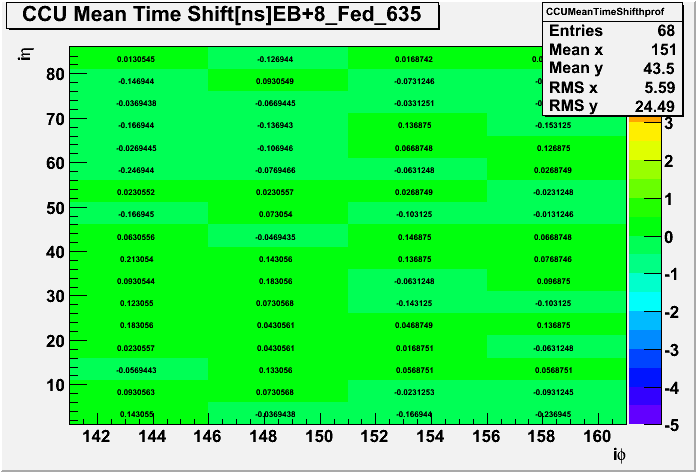
\includegraphics[height=0.45\textwidth, width=0.45\textwidth]{THESISPLOTS/CCU_Mean_Time_ShiftEB_Plus8_Fed_635.png} \quad
%%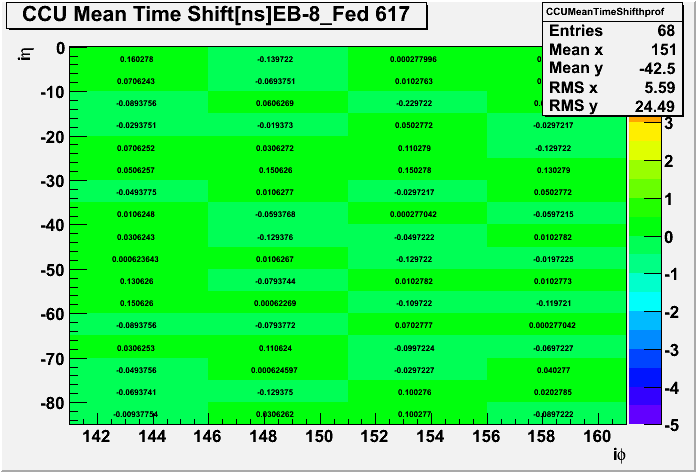
\includegraphics[height=0.45\textwidth, width=0.45\textwidth]{THESISPLOTS/CCU-Mean-Time-Shift-EBMinus8-Fed617.png}}

%%\vspace{1cm}
%%\mbox{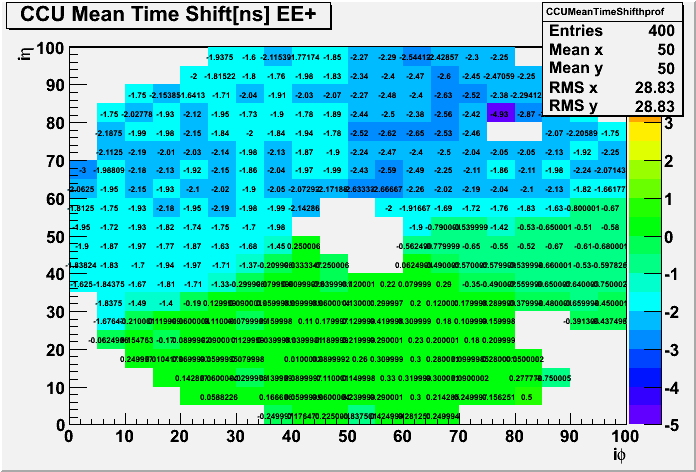
\includegraphics[height=0.45\textwidth, width=0.45\textwidth]{THESISPLOTS/CCU_Mean_Time_Shift_EEP_Laser.png} \quad 
%%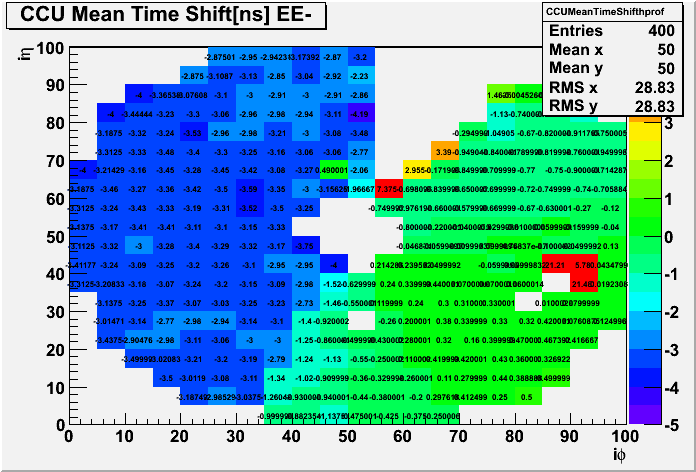
\includegraphics[height=0.45\textwidth, width=0.45\textwidth]{THESISPLOTS/CCU_Mean_Time_Shift_EEM_Laser.png}}
%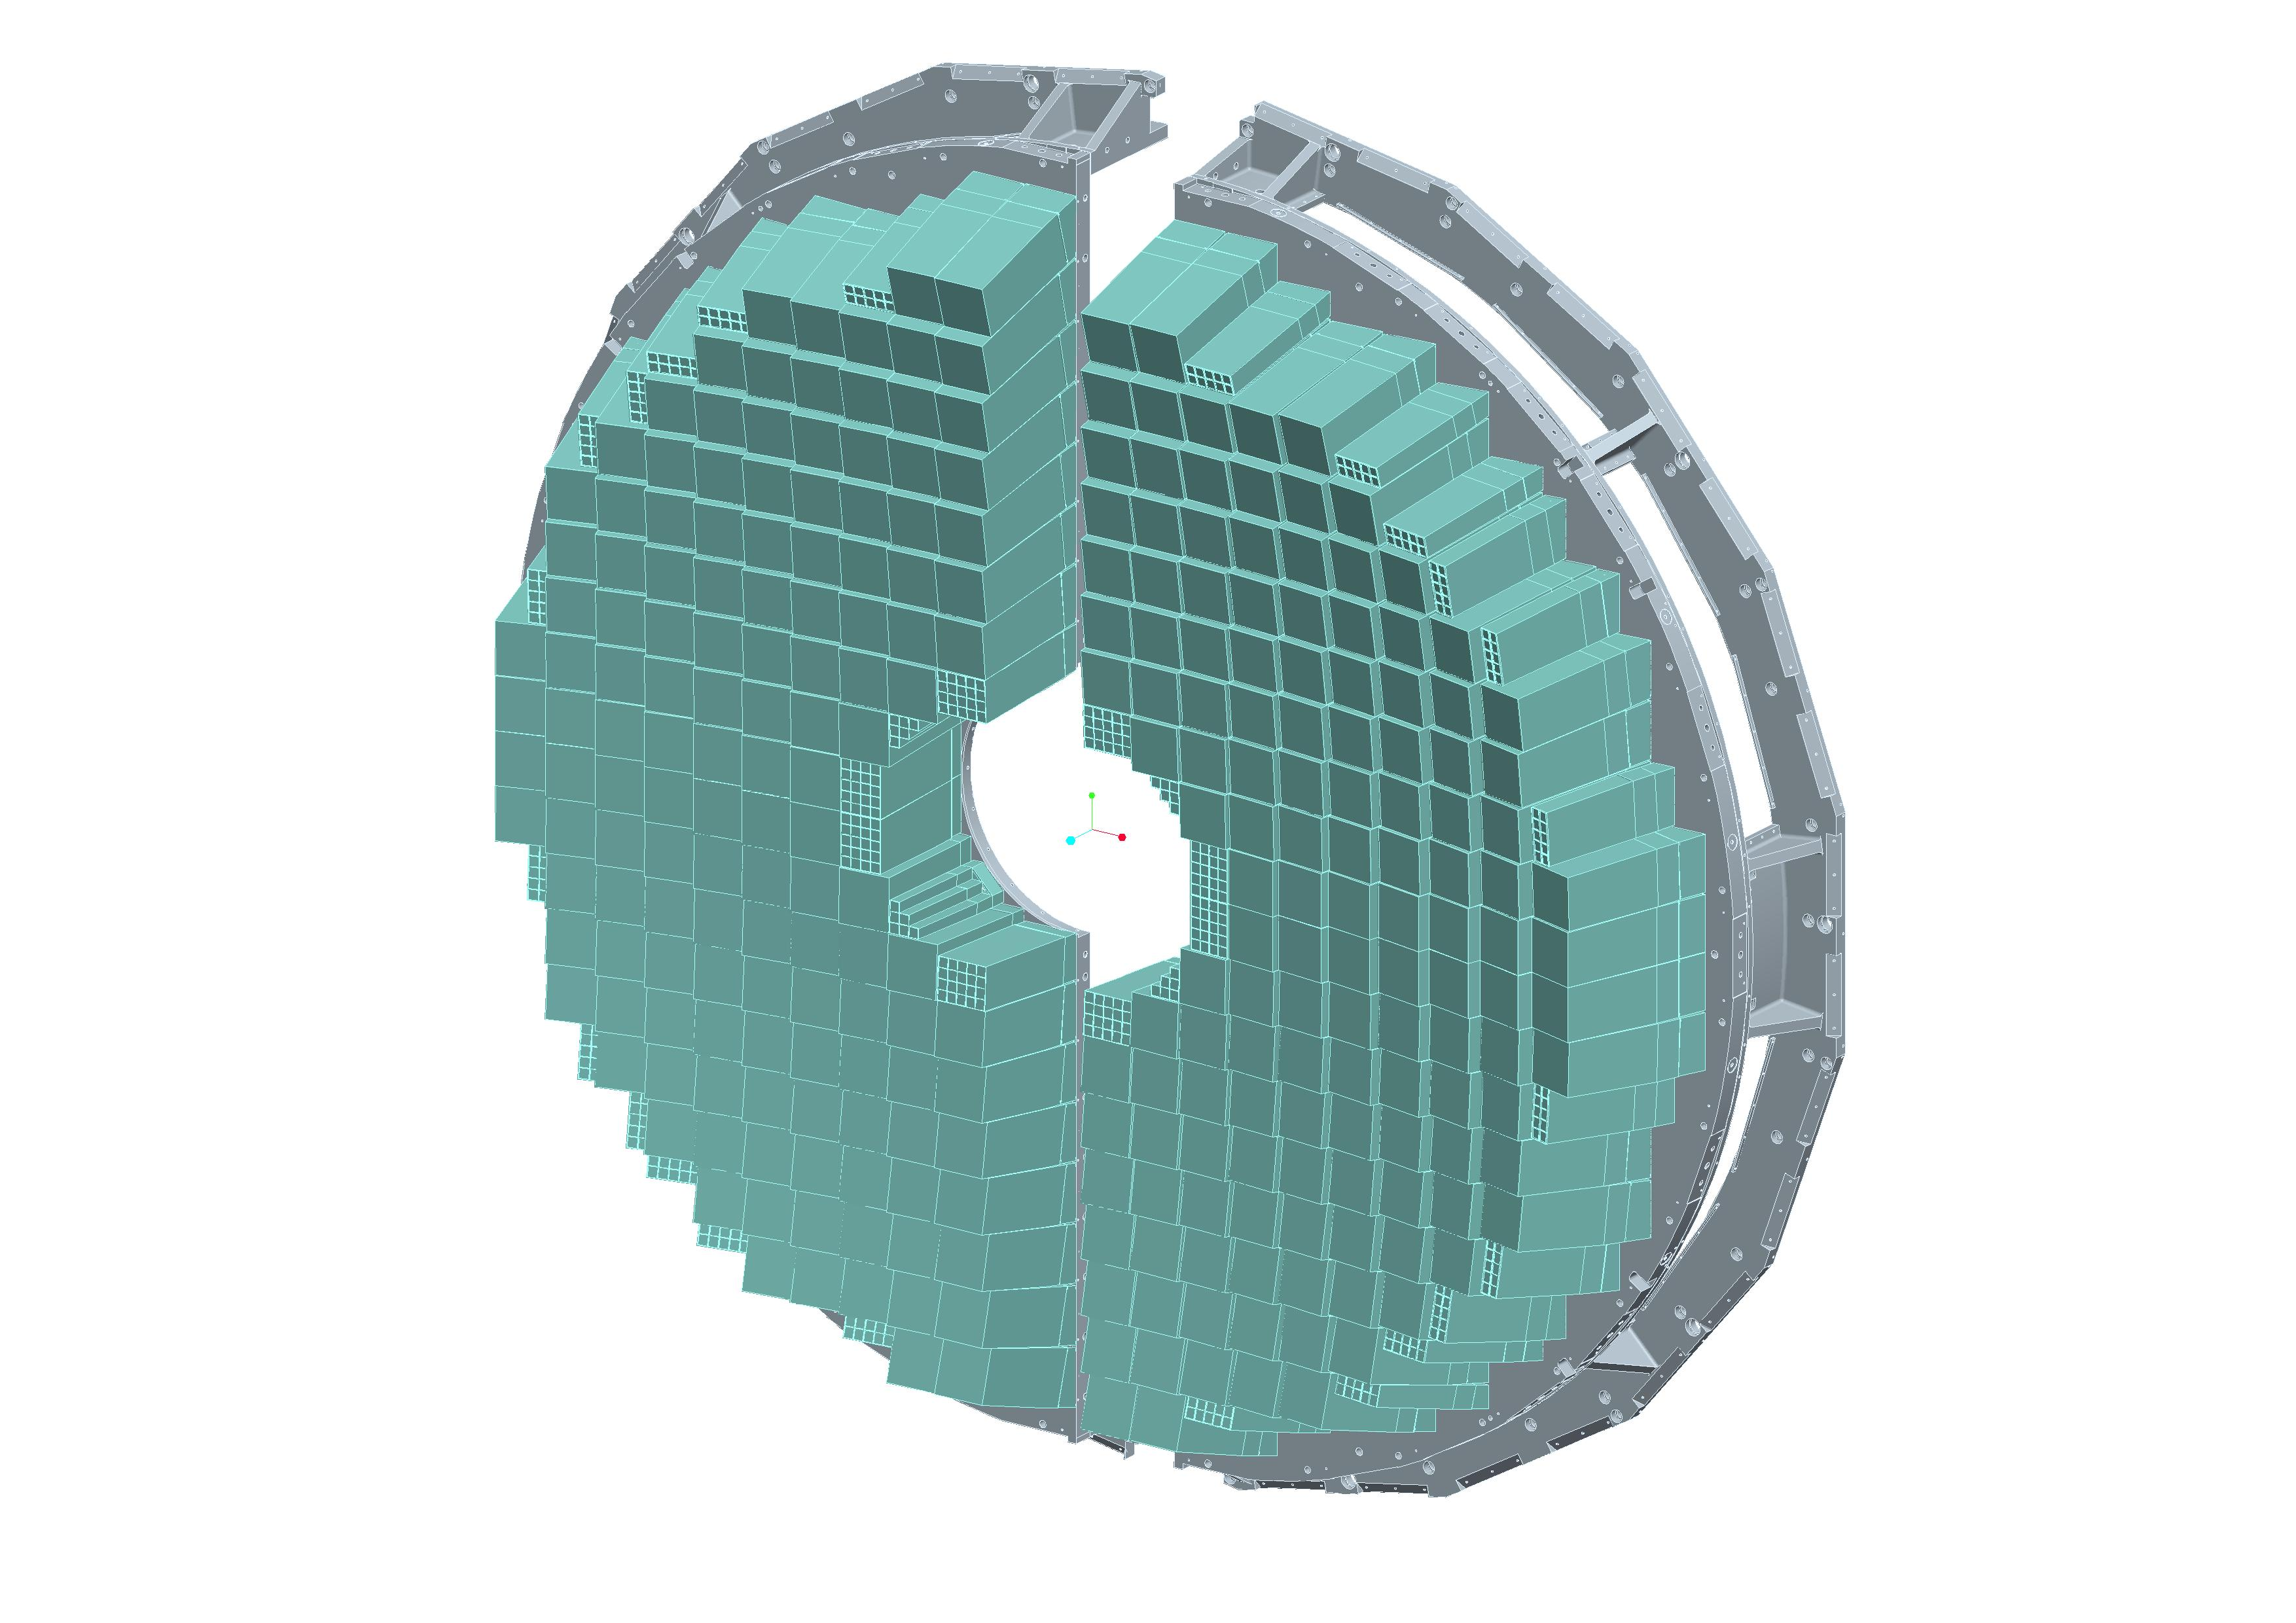
\includegraphics[scale=0.06]{THESISPLOTS/endcap_CMS.png}} 
%%\captionof{figure}{\textit{Top}: The mean time distribution obtained from laser of crystals in a single FED \ie EB$\pm$8. 
%%\textit{Bottom}: Clock and Control Unit ~(CCU) mean time shift distribution of FEDs EE$+$ and EE$-$. 
%%$\Delta t_{CCU}$ distributions after the global shift has been removed. The adjustment for global time shift per FED due to difference in light source for each CCU has been shown to reduce the possibility of CCU showing false time shift. }
%%\label{fig:TimeLaser}
%%\end{center}
%%%%%%%%%%%%%%%%%%%%%%%%%%%%%%%%%%%%%%%%%%%%%%%%%%%%%%%%%%%%%%%%%%
\subsection{Time Bias}
%%%%%%%%%%%%%%%%%%%%%%%%%%%%%%%%%%%%%%%%%%%%%%%%%%%%%%%%%%%%%%%%%%
An additional source contributing to poor time measurement arise from energy related time bias. This bias originates from the time reconstruction algorithm. Is is expected that the ratio approach for time reconstruction performs efficiently for all ADC counts. However, during data recording in LHC Run 1, it was observed that for high ADC counts produced by very energetic particles, an inherent bias in the time is introduced by the multi-gain pre-amplifier electronics for electromagnetic particles with energy above certain gain transition points. 
%The energy  deposited by an incoming particle on a crystal is recorded as an ADC count, $A$, which is the signal amplitude of the recorded pulse shape. This ADC count can be converted into energy in \GeV through some conversion factors and adjustments. 
The full conversion of the energy of a particle recorded by a crystal in ADC counts to \GeV is expressed as; $    E_{i} =  G \cdot S_{i}(t) \cdot C_{i} \cdot A_{i}$, where $A$ is the amplitude from the pulse shape in ADC counts, $G$ is the ADC-to-GeV conversion factor equal to $0.039$($0.063$) in EB(EE), $C_{i}$ is the inter-calibration coefficients accounting for individual channel response to the electromagnetic shower and $S_{i}(t)$ is the correction term obtained from laser accounting for radiation-induced channel response.  $S_{i}$ changes over time.
The first gain transition point~(Gain-1) of the multi-gain pre-amplifier occurs at $4096$~ADC counts corresponding to $159.744$~\GeV in EB and $258.048$~\GeV in EE. The subsequent Gain~6 and 12 transitions occur at energy values of \TeV.
\newline
The ratio algorithm introduced time bias at gain transition points which need to be adjusted.
These adjustments are made on an energy dependent basis during event reconstruction for a particular CMS event reconstruction software~(CMSSW) release. Figure \ref{fig:TimeBias} shows the comparison between two CMS event reconstruction software releases, CMSSW44X, where these time bias corrections have not been  made and CMSSW53X, where the the corrections have been made. Evidently, the average time displayed in both CMSS44X and CMSS53X show the disappearance of the time bias for all particle energy in CMSSW53X after the time bias corrections were made.
%The bias in timing introduced by these gain transitions cannot be calibrated at hardware, so we developed a method of adjusting the
%timing measurements for the timing bias at the CMS event reconstruction level.
%Using reconstructed hits with similar selection as our offline timing calibration, selected hits are also required to be part of a basic cluster~(usually $3\times 3 $ or $5\times 5$ matrix of crystals). These hits must have amplitude with channel noise consideration above $10$ ADC counts. We reject hits with very large timing biased and large swiss-cross variable beyond our selection threshold~(0.99). A distribution of the hit time against its amplitude is plotted and then sliced in bins of amplitude. Bins containing at least 7 hits are fitted using a Gaussian function constrained within $\pm 7$~ns. The average(mean) and standard deviation(RMS) from these distributions is plotted against their corresponding amplitude or energy to give a distribution of mean and standard deviation  against amplitude. This procedure is performed for different \textit{Modules} or pseudo-rapidity~($\eta$) range starting from $\eta = 0$ which is \textit{Module}~1 in barrel to $\eta = 3$ for high-eta in endcap.
%Figure \ref{fig:TimeBias} shows the mean against energy distribution for different reconstruction CMS Software~(CMSSW) release versions where these timing bias corrections have been applied~(CMSSW5XY) and have not been applied~(CMSSW44X) during object reconstruction. 
%It is now a standard procedure in CMS that these timing biases are applied for all CMS releases. %All CMSSW releases beyond CMSSW5XY now have these bias corrections applied. 
%The dataset used for this reconstruction is the \textit{DoubleElectron} and \textit{Photon} dataset processed using CMSSW44X release during LHC RUN 1 and later reprocessed using CMSSW53X with the bias corrections applied. 
\begin{center}
\centering
\mbox{
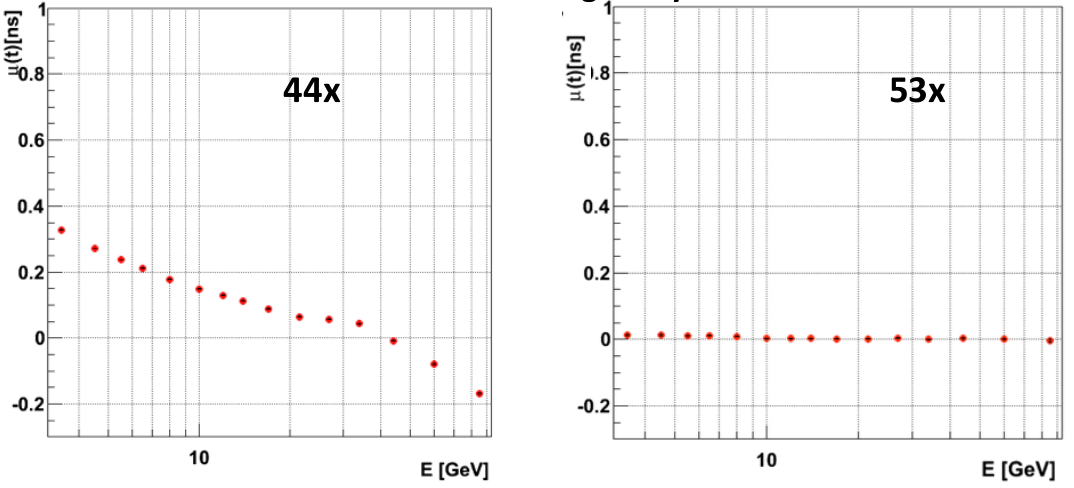
\includegraphics[height=0.450\textwidth, width=0.85\textwidth]{THESISPLOTS/AmplitudeVsTimeCMSSW_Comparison.png} } 
\vspace{5cm}
\mbox{
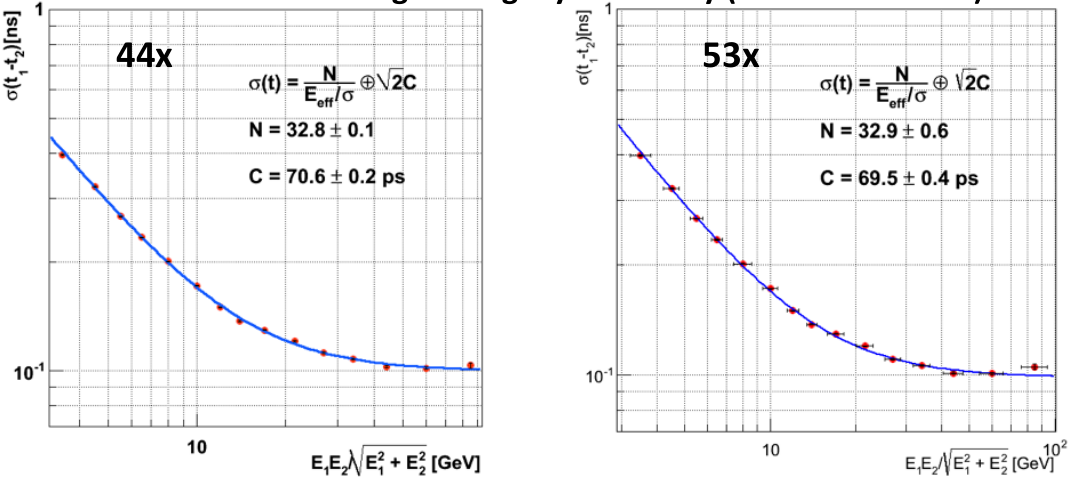
\includegraphics[height=0.460\textwidth, width=0.85\textwidth]{THESISPLOTS/TimingResolutionCMSSW_Comparison.png}
}
\vspace{-5cm}
\captionof{figure}{Distribution of mean time~($\mu$,\textit{top row}) and time deviation~($\sigma$, \textit{bottom row}) as a function of crystal energy for EB prior~(left) and after~(right) time bias corrections depending on energy have been applied.}
\label{fig:TimeBias}
\end{center}

%%Additional sources of Time bias
\paragraph*{}
To investigate further for any additional time bias un related to the particle energy, we study how the crystal geometric position in ECAL covering from $\eta = 0$ to $\eta = 3.142$. The results shown in Figure \ref{fig:EtaDep} show no crystal position or $\eta$ dependence. However, time bias of the order of 100~ps have been observed.
There are efforts to understand the source of these time bias with speculations that the time bias might be caused by electronics or loss in \pb crystal transparency due to radiation.
% and over time, which in the this case we use the proton-proton collision run period~(RUN Number)
%There are other timing biases of the order of about 100~ps have been observe in the difference in time for crystals belonging to different electronics. Such timing bias are not yet understood.

%We have also performed detail studies to check for $\eta$ and run dependence contributions to the timing bias. 
%In figure \ref{fig:EtaDep}, we show the distribution of the mean time~($\mu$) and standard deviation~($\sigma$) for different modules in different resgions in barrel and sections in endcap. The timing resolution do not show any dependence on pseudo-rapidity~($\eta$), however 
\begin{center}
\centering
%\mbox{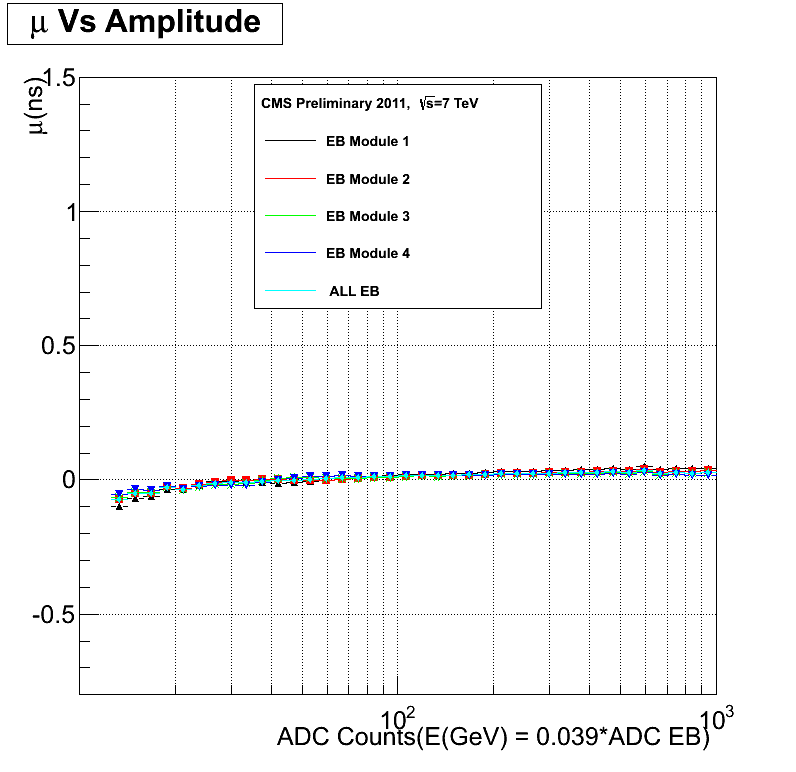
\includegraphics[height=0.45\textwidth, width=0.45\textwidth]{THESISPLOTS/EB_TimeVsAmplitude_StabilityCMSSW_5_3_X.png} \quad
%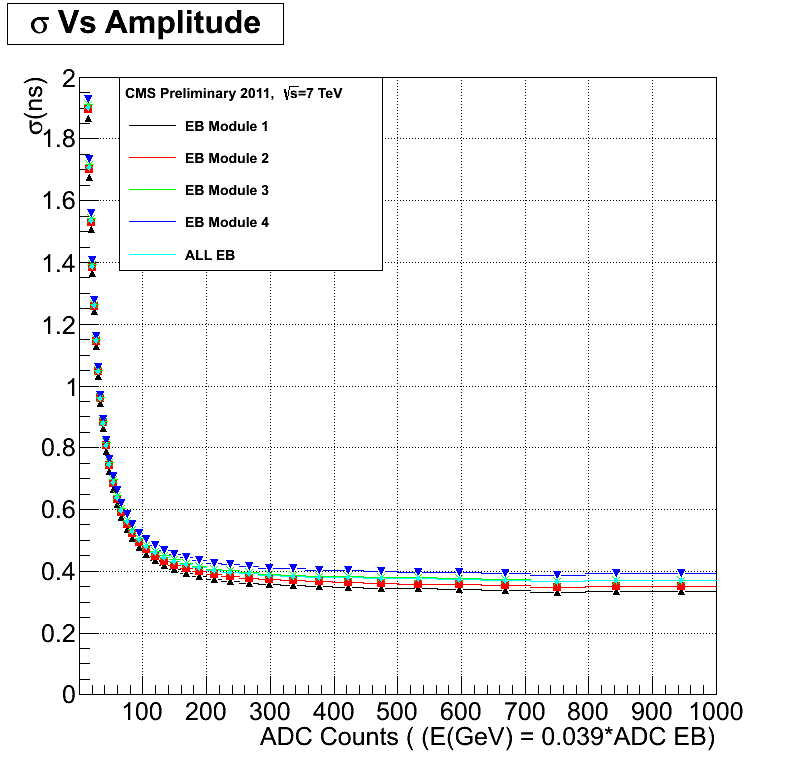
\includegraphics[height=0.45\textwidth, width=0.45\textwidth]{THESISPLOTS/EB_SigmaVsAmplitude_Stability_In_CMSSW_53X.png}}
%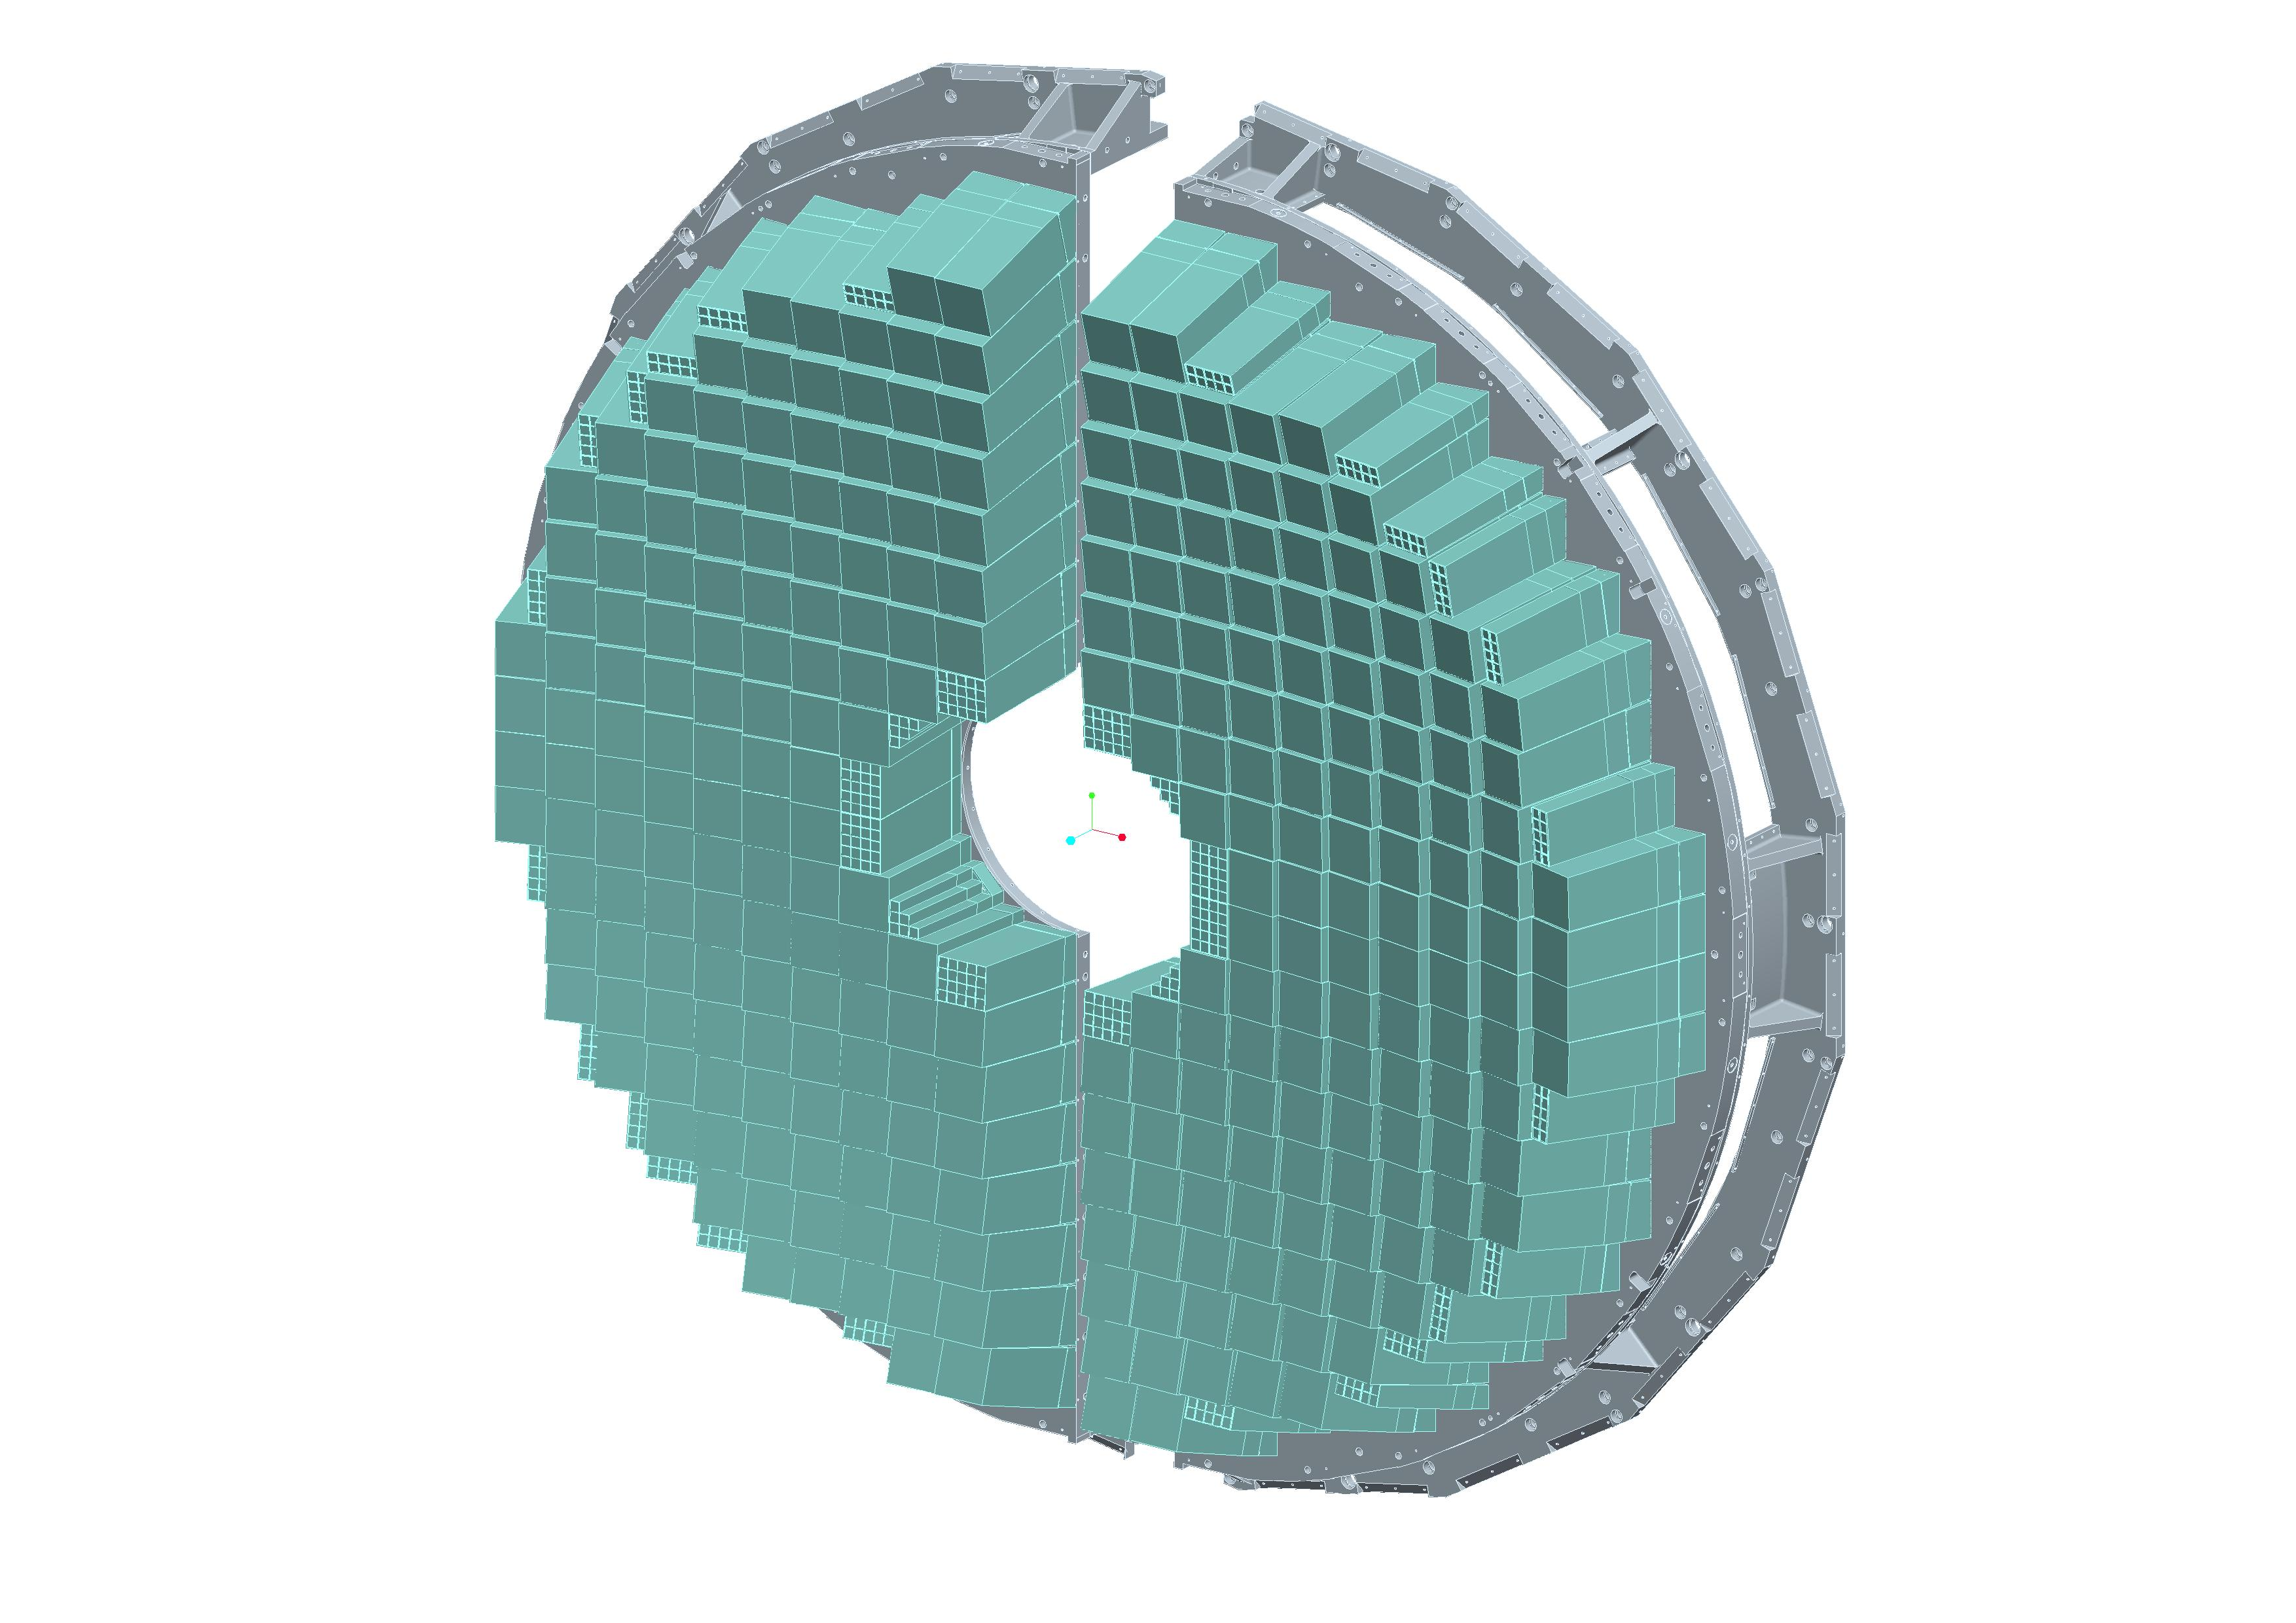
\includegraphics[scale=0.06]{THESISPLOTS/endcap_CMS.png}} 
%\vspace{-0.5cm}
\mbox{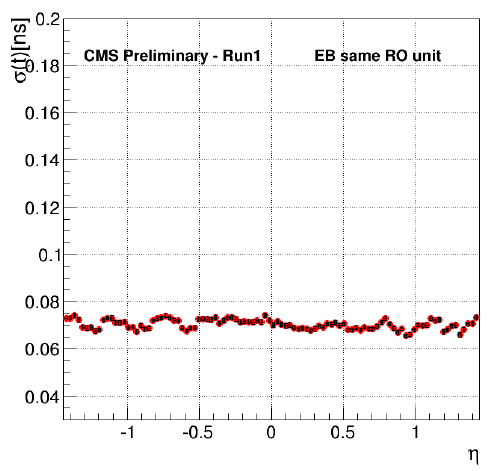
\includegraphics[height=0.60\textwidth, width=0.80\textwidth]{THESISPLOTS/TimeResolution_Vs_Eta.png}}
%\mbox{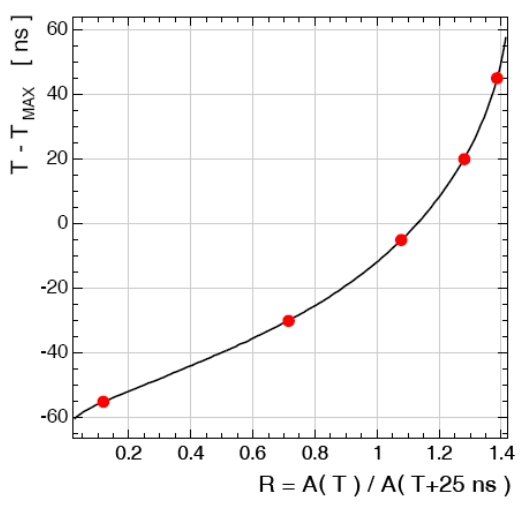
\includegraphics[scale=0.45]{THESISPLOTS/TMaxPhaseVsRatio.png}}
%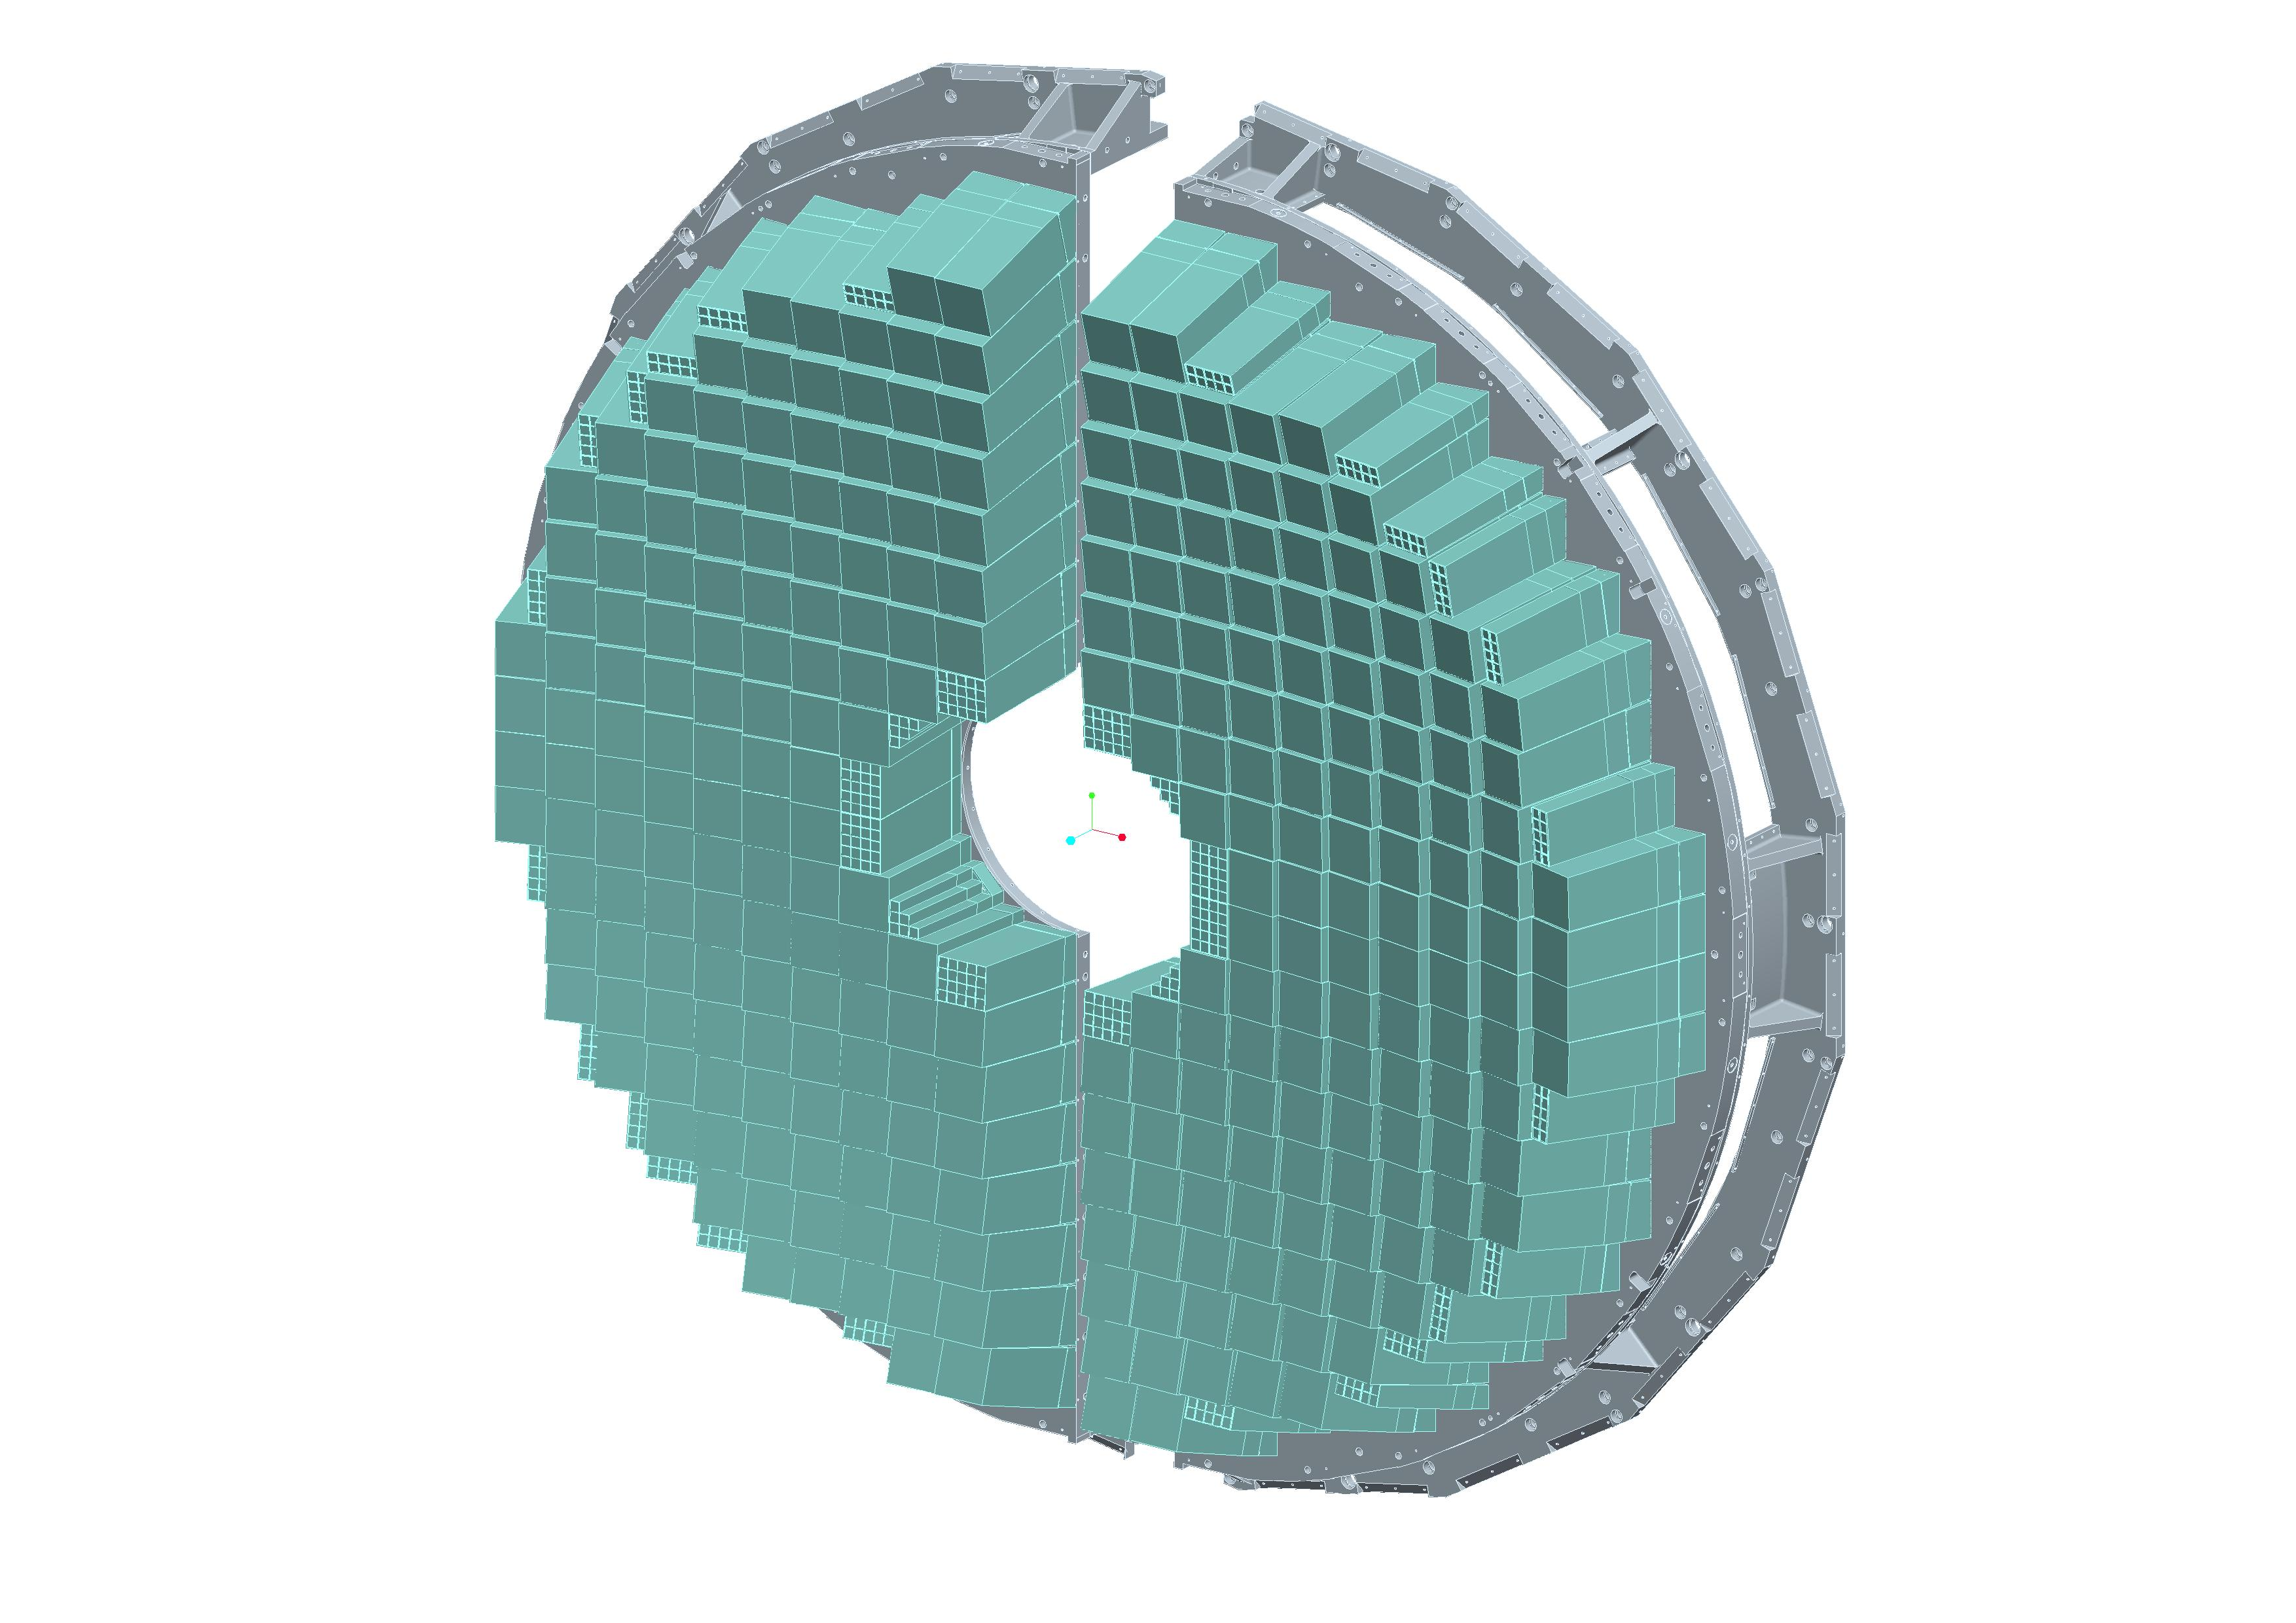
\includegraphics[scale=0.06]{THESISPLOTS/endcap_CMS.png}} 
%\captionof{figure}{\textit{Top row}: Distribution of mean time~($\mu$) as a function of amplitude~(left) and resolution~($\sigma$) as a function of amplitude~(right) for different pseudo-rapidity regions in the barrel. ~\textit{Bottom}: All modules in EB combined timing resolution as a function against $\eta$ crystals in the same readout electronics in  barrel~(EB).}
\captionof{figure}{Distribution of the time standard deviation~($\sigma$) against crystal geometrical position, $\eta$, in the ECAL barrel. Almost flat distribution of $\sigma$ with $\eta$. }
\label{fig:EtaDep}
\end{center}
%\clearpage
%%%%%%%%%%%%%%%%%%%%%%%%%%%%%%%%%%%%%%%%%%%%%%%%%%%%%%%%%%%%%%%%%%
%%%%%%%%%%%%%%%%%%%%%%%%%%%%%%%%%%%%%%%%%%%%%%%%%%%%%%%%%%%%%%%%%%
\subsection{ECAL Time Performance With Z Bosons}
%%%%%%%%%%%%%%%%%%%%%%%%%%%%%%%%%%%%%%%%%%%%%%%%%%%%%%%%%%%%%%%%%%
%Timing calibration is performed to properly align the time of an incoming event which can be misaligned because of poor inter-calibration between different front end electronics, biased on timing due to timing dependence on energy, reduction in \pb crystal transparency due to radiation, hardware intervention during machine repairs and other effects. To measured 
We evaluate the precision of ECAL time measurements during proton-proton collisions by studying the time measurement of a well understood physics process; the decay of the \PZ boson to an electron pair, \ie $\PZ \rightarrow \Pelectron \Ppositron$.
%We study the performance of timing measurements by ECAL crystals using well studied physics processes like the decay of a $\PZ$ boson to an electron pair, \ie $\PZ \rightarrow \Pelectron \Ppositron$. 
We use the standard deviation~(time resolution), $\sigma_{eff}$, of the difference in arrival time of the two electrons to evaluate ECAL time performance.
The standard deviation is obtained from the difference in the seed time ,$t_{seed}$, of the electron electromagnetic shower of each electron after correcting for contributions from the bending of the electron travel path inside CMS magnetic field of 3.8~T.  
% gives a good estimate of the timing resolution performance of the ECAL crystals.
In Figure \ref{fig:ZeeTimePerformance2}, we present the distribution of the  time difference, $t_{electron1} - t_{electron2} = t_{seed1}-t_{seed2}$, of both electrons adjusted for time of flight corrections and in Figure \ref{fig:ZeeTimePerformance1}, we show the time resolution or  $\sigma_{eff}(t_{1} - t_{2})$, obtained from the time distribution of the seed crystal time without correcting for the bending of the electron's flight path contributions. A time resolution of $232$~ps in EB and $384$~ps in EE is realized. However, if we remove the contributions from the spread in time, $\sigma(t_{colision})$, due to the finite time it takes for the two proton bunches of length $5.5$~cm to collide; which is about $\sigma(t_{colision}) = \sigma(t_{Z}) = 183~ps$, we obtain an improved time resolution of $142$~ps in EB and $337$~ps in EE. The selection for \PZ candidate events required that the electrons have a transverse energy bigger than 10~\GeV  and the reconstructed \PZ mass is within, $ 60~GeV < m_{inv}(e_{1},e_{2}) < 150~ GeV$ in order to ensure  mostly good $\PZ$ boson candidate events are used. 
%difference in the arrival time of both electrons at ECAL crystals, which in principle
%should be zero, to evaluate ECAL timing measurement performance. This performance is expressed by using the standard deviation, $\sigma_{eff}$, of the difference in arrival time of both electrons.
%The decay of a $\PZ$ boson is well understood and effects due to poor event reconstruction or detector effects are well measured. 
%The idea is to use the two electrons which in principle should have the equal arrival time  and use their measured time difference to estimated the timing resolution performance of the \pb crystals in ECAL. In order to understand different source of poor timing measurements, we study the following different methods for measuring the time of the two electrons:
%The crystal arrival time for each electron is the time of the seed crystal~($t_{seed}$) of the electron energy super cluster.

% using the time of the seed crystal~(crystal with highest energy) in the electron suspercluster and
%\begin{enumerate}
%\item The time of two crystals in a single electron super cluster.
%\item Neighboring crystals in a single electron supercluster sharing the same supercluster energy. This has the advantage of minimizing shower propagation effects.
%\item Two crystals each from the different electron superclusters.
%\item Two well reconstructed and energy corrected superclusters of each electron in the $\PZ$ decay. 
%\end{enumerate}

%Here are additional sources of contributions to the electron time which we take into consideration:
%\begin{enumerate}
%\item The bending of the electron path due to the presence of the $3.8$~T magnetic field of the CMS detector.
%Despite this good timing resolution of about $232$~ps in EB and $384$~ps in EE, there are other sources contributing to poor timing resolution compared to test beam results of $\leq 100$~ps. These sources include,
%displaced collisions because "partons"~(quarks inside a proton) in the proton bunches did not collide at exactly the same nominal interaction point~(IP), the fact that proton-proton collisions developed over the full duration due to overlap of the proton bunches and timing biases from different electronics and crystal-to-crystal intercalibration.
% This causes a spread in collision timing and account for about $183$~ps in worsening of timing resolution measurements.


%In the time calibration algorithm, the photon flight path is a straight path from IP to ECAL crystal. However, for electrons, being charged particles moving in the presence of a magnetic field, this is not the case. In addition to flight path, there are slight variations due to differences in the vertex position of electrons. Since it is possible to reconstruct the true vertex position of the electron, these small Time Of Flight~(TOF) variations can be corrected. On the other hand this is not possible for photons as it is almost impossible to know its true vertex position. There are active investigations on how to reconstruct the true primary vertex of a photon using information of its arrival time in the ECAL, cluster position and energy. This study is motivated by Higgs decay.
 
%In summary, we use photons for timing calibration studies and electrons for studying the timing performance.
%Without adjusting for contributions from individual proton collisions across the entire proton bunch luminous region of nearly $5.5$~cm(referred here as \textit{proton collision time} of about $\sigma(t_{colision}) = \sigma(t_{Z}) = 183~ps$) the measured ECAL timing resolution is $232$~ps in EB and $384$~ps in EE. When adjusted for this contribution, the timing resolution is about $142$~ps for EB and $338$~ps in EE.

\begin{center}
%\begin{figure}
\centering
\mbox{
\includegraphics[height=0.5\textwidth, width=0.45\textwidth]{/home/tensr/Documents/ECAL_NOTES/PLOTS/2013/ECALTDRPLOTS/EB-EB-TOF-Corr-difference-of-seed.png}\quad
\includegraphics[height=0.5\textwidth, width=0.45\textwidth]{/home/tensr/Documents/ECAL_NOTES/PLOTS/2013/ECALTDRPLOTS/EE-EE-TOF-Corr-difference-of-seed.png}}
\captionof{figure}{Ecal time difference between the two reconstructed electrons in $\PZ \rightarrow \Pelectron \Ppositron$ decay. The electron time is the seed~(crystal with highest energy deposit) time with additional correction due to the time of flight of the electron in EB and EE} 
\label{fig:ZeeTimePerformance2}
%\end{figure}
\end{center}

\begin{center}
\centering
\mbox{
\includegraphics[height=0.5\textwidth, width=0.45\textwidth]{/home/tensr/Documents/ECAL_NOTES/PLOTS/2013/ECALTDRPLOTS/EB-EB-Time-of-seed.png}\quad
\includegraphics[height=0.5\textwidth, width=0.45\textwidth]{/home/tensr/Documents/ECAL_NOTES/PLOTS/2013/ECALTDRPLOTS/EE-EE-Time-of-Seed.png}}
%\vspace{-1cm}
\captionof{figure}{Ecal absolute time of a single reconstructed electron in $\PZ \rightarrow \Pelectron \Ppositron$ decay. The electron time is the seed~(crystal with highest energy deposit)time of the electron in EB and EE} 
\label{fig:ZeeTimePerformance1}
\end{center}


%To compare the timing resolution obtain during test beam studies to that obtained at the end of LHC Run 1, a similar figure is made shown in figure \ref{fig:ZeeTimeResolution} produced from the $\PZ \rightarrow \Pelectron \Ppositron$ decay events with the time difference between the two electrons plotted as a function of the effective amplitude normalized to the noise in ECAL barrel for LHC Run 1. The noise term in consistent with results obtained during test beam while the constant term is about $150$~ps, much larger than test beam results~($70$~ps). Its has been shown that effects such as poor inter-calibration between two different front end electronics, run dependence and radiation might be the reason for this large constant term. Figure \ref{fig:ZeeTimeResolution}(\textit{left}) show the time resolution against effective amplitude with the constant term $\bar{C} = 67$~ps if both crystals are from the same front end electronics  while figure \ref{fig:ZeeTimeResolution}(\textit{right} is the time resolution against effective amplitude with $\bar{C} = 154$~ps if both crystals are from different readout unit or trigger tower. The noise term $N$ is the same as test beam for both measurements This indicates an effect due to different inter-calibrations for different electron shower initiation points in different trigger towers.
\paragraph*{}
We also investigate the contributions attributed to the readout electronics on the time resolution using events with $\PZ \rightarrow \Pelectron \Ppositron$ decay.
Figure \ref{fig:ZeeTimeResolution}(left), shows the time resolution obtained from measuring the electrons arrival time in the case where the seed crystal time of both electrons is read from the crystals belonging to same ReadOut~(RO) electronics  and compared to the other case where the seed crystal time is read from crystals belonging to two different readout electronics shown in Figure \ref{fig:ZeeTimeResolution}(right).
The Constant term, $C$, for the same RO electronics is about $67$~ps while that for different RO electronics is $130$~ps indicating that electronic readout de-synchronization contributes to the worsening of the time resolution.
\paragraph*{} 
Despite, the observed 100~ps bias which seems to be related to readout electronics, we argue that, with a time resolution of $\sigma(t) \leq 400$~ps, the ECAL subdetector is very reliable for time measurements and can be used in the search for delayed electromagnetic particles produced in the decay of long-lived particles.
\newline
The ECAL time resolution for the entire LHC Run 1 of 2011 and 2012, comparing the absolute and single precision time measurements is summarized in table \ref{tab:TIMERes}.% The results presented were obtained studying the time measurements of events with  $\PZ \rightarrow \Pelectron \Ppositron$ decay.

%the comparison of ECAL timing resolution obtained using events with $\PZ \rightarrow \Pelectron \Ppositron$ the case where both crystals belong to different frontend electronics~(\textit{right}) to where both crystals belong to the same electronics(\textit{right}) and observe the $100$~ps bias due to different electronics. The timing resolution from LHC RUN1 shown in figure \ref{fig:ZeeTimeResolution} compared to timing resolution from test beam shown in figure \ref{fig:FitTimeRes}, shows that we are yet to achieve the level of ECAL timing resolution obtained during test beam. Nevertheless, the current timing resolution of $\sigma(t) \leq 400$~ps is good for using ECAL timing measurements to study physics processes with photons and electrons produced from the decay of long-lived particles.
%Table \ref{tab:TIMERes} shows the summary of the ECAL timing resolution comparing the absolute and single precision timing resolution studied using events with \PZ decay for 2011 and 2012 of the entire LHC Run 1. 
%\vspace{-2cm}
\begin{center}
%\begin{figure}
\centering
\mbox{
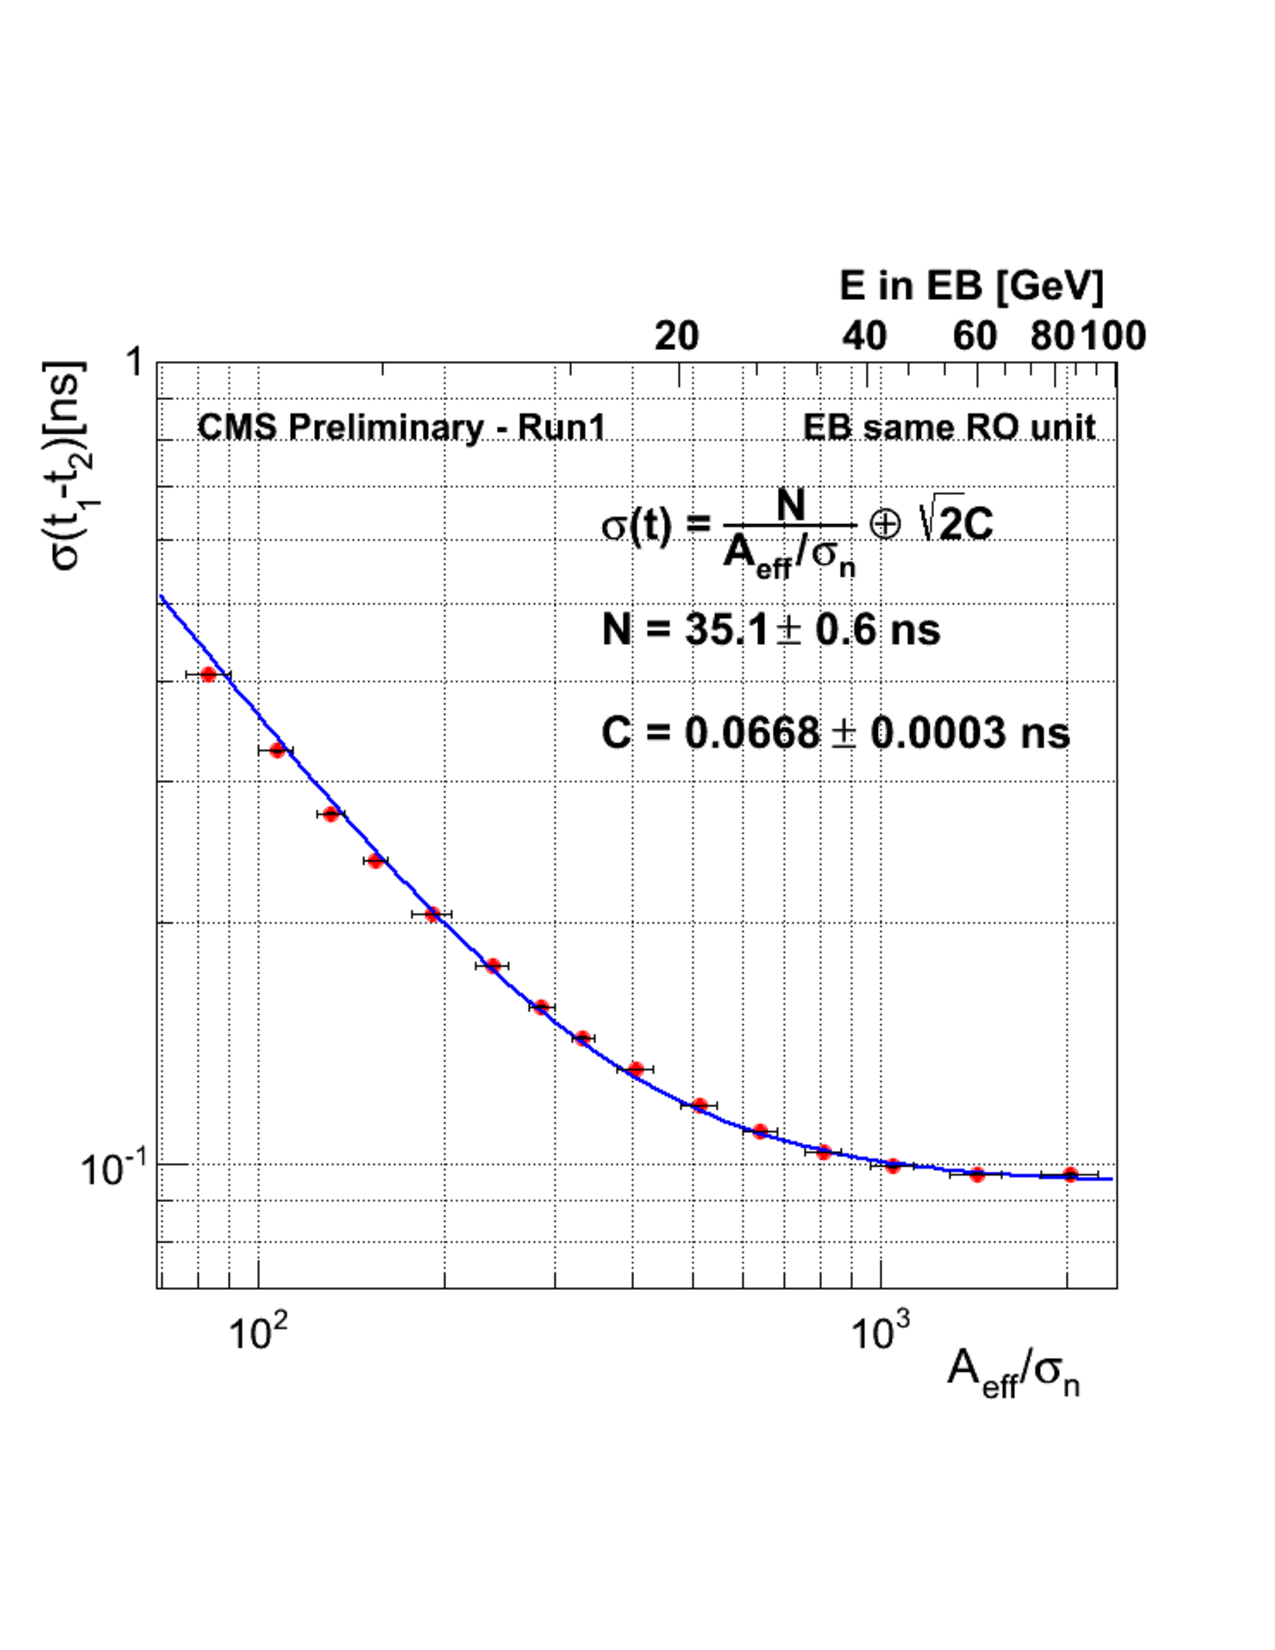
\includegraphics[height=0.70\textwidth, width=0.5\textwidth]{THESISPLOTS/TimeResSameElecCrystals.pdf}\quad
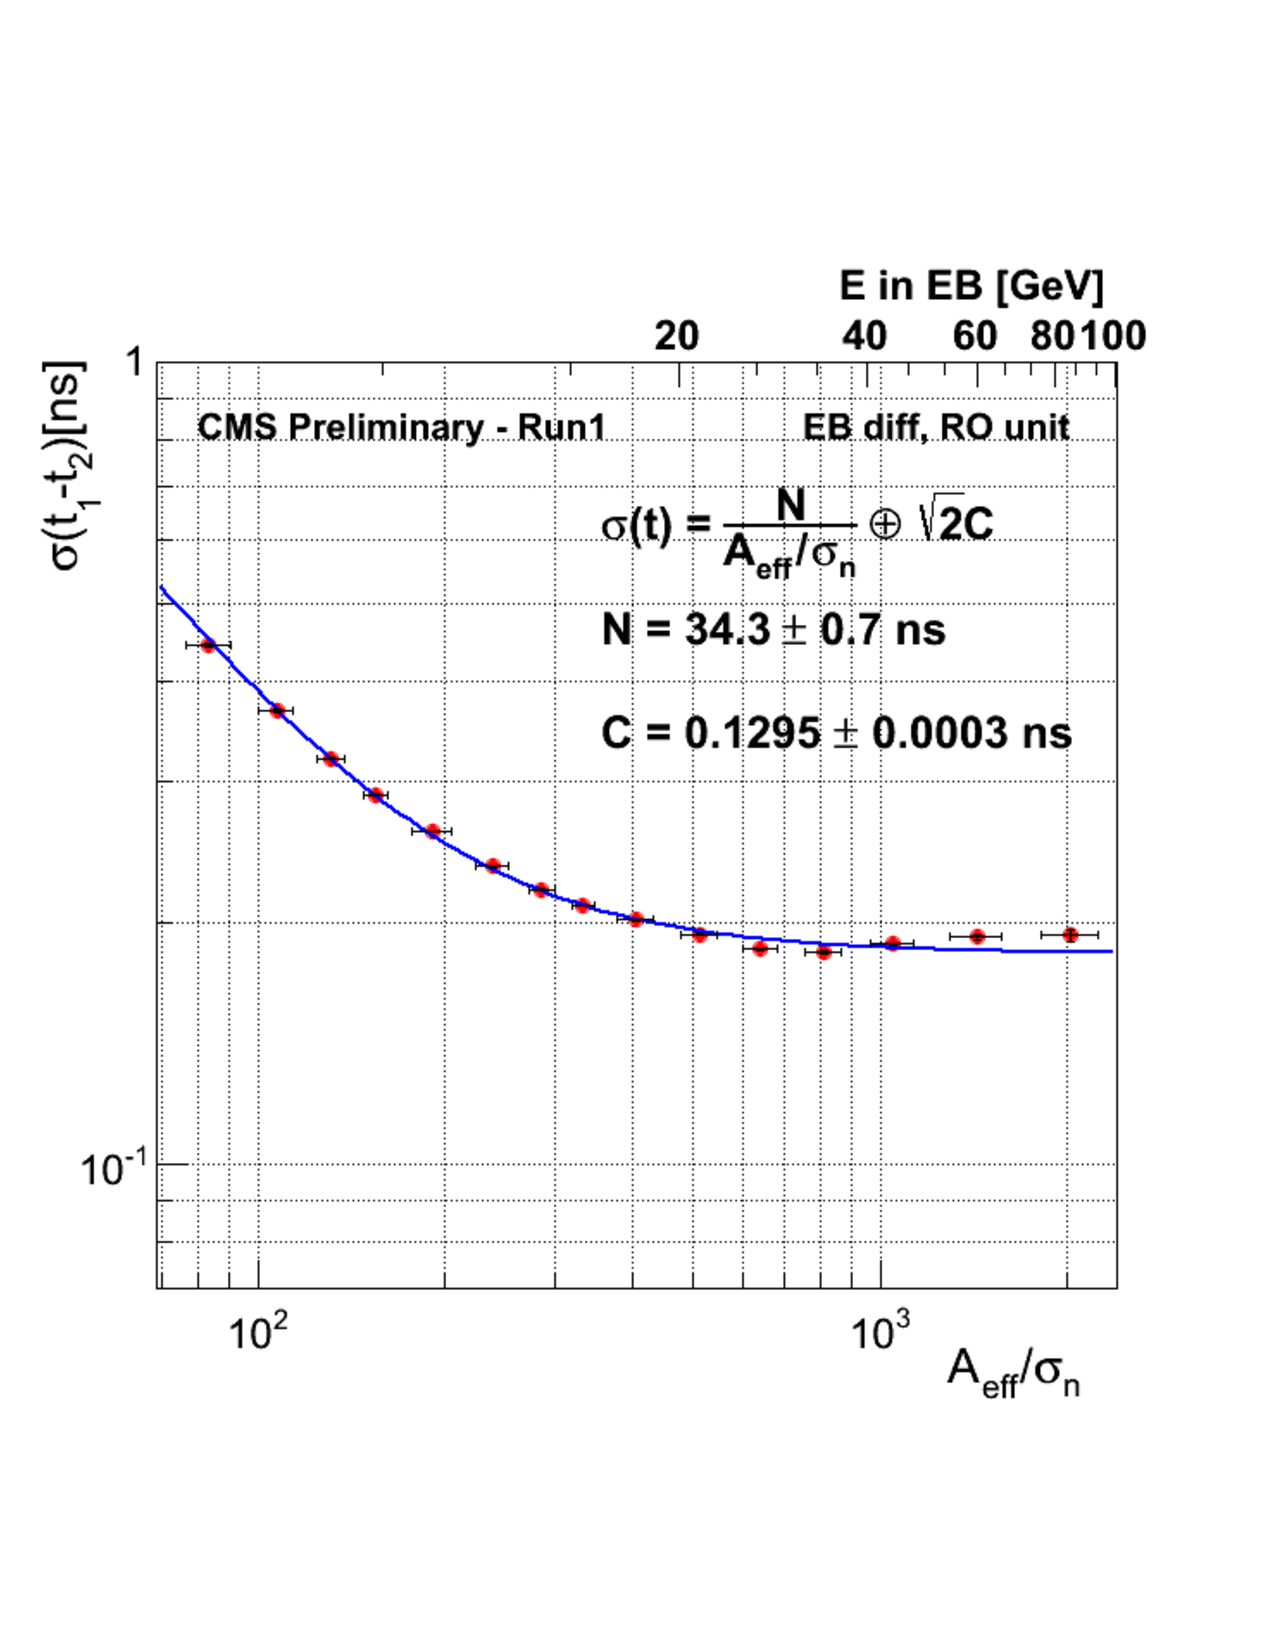
\includegraphics[height=0.70\textwidth, width=0.5\textwidth]{THESISPLOTS/TimeResDiffElecCrystals.pdf}}
\vspace{-2.5cm}
\captionof{figure}{ Timing resolution from:
\textit{left}: Two most energetic crystals in the same readout unit,
\textit{right}: Two most energetic crystals belonging to different readout units,
as a function of effective amplitude($A_{eff} = A_{1}A_{2}/\sqrt{A^{2}_{1} + A^{2}_{2}}$) normalized to noise in EB.
Both crystals are from reconstructed electrons in  $\PZ \rightarrow \Pelectron \Ppositron$ events.} 
\label{fig:ZeeTimeResolution}
%\end{figure}
\end{center}

%\paragraph*{Summary}
%Table \ref{tab:TIMERes} shows ECAL timing resolution for 2011 and 2012 LHC Run 1. 
\begin{center}
%\begin{table}
\centering
 %\setlength{\abovecaptionskip}{0pt}
  %\setlength{\belowcaptionskip}{10pt}
 %\topcaption{GMSB,GGM Phenomenology and Relevant final states}
  \begin{tabular}{cc||lc} % p{0.1cm}|p{0.1cm}|}
  %\hline
 & \multicolumn{1}{r}{\bfseries{ECAL Timing Resolution}}\\
  \toprule
  \hline
 & \multicolumn{2}{c}{\bfseries{2011}} \\
   \hline \hline
   & \vtop{\hbox{\strut{\bfseries{Absolute Time}}} \hbox{\strut{$\sigma_{eff}(t_{seed})$[ps]}} }  
   & \vtop{\hbox{\strut{\bfseries{Single Precision}}}\hbox{\strut{$\sigma_{eff}(t_{e1} - t_{e2})/\sqrt{2}$[ps]}} } \\ \hline
   \textbf{EB} & 376  & 190 \\
      \textbf{EE} & 356  & 282 \\
      \hline 
& \multicolumn{2}{c}{\bfseries{2012}}  \\
   \hline \hline
   &  \vtop{\hbox{\strut{\bfseries{Absolute Time}}}\hbox{\strut{$\sigma_{eff}(t_{seed})$[ps]}} }       
   &  \vtop{\hbox{\strut{\bfseries{Single Precision} }} \hbox{\strut{$\sigma_{eff}(t_{e1} - t_{e2})/\sqrt{2}$[ps]}} }  \\ \hline
   \textbf{EB} & 340  & 164 \\
      \textbf{EE} & 342  & 272 \\
      \hline
      \bottomrule
  \end{tabular}
   \captionof{table}{ECAL timing resolution absolute time and single precision for 2011 and 2012 of LHC Run 1}
 %\caption{ECAL timing resolution performances for 2011 and 2012 of LHC Run 1}
 \label{tab:TIMERes} % for use in \ref{table1} if you want to refer to the table number
\end{center}
%\end{table}
%\begin{center}
%\begin{tabular}{cc|c|c|c|c|l}
%\centering
%\cline{3-6}
%& & \multicolumn{4}{ c| }{Primes} \\ \cline{3-6}
%& & 2 & 3 & 5 & 7 \\ \cline{1-6}
%\multicolumn{1}{ |c| }{\multirow{2}{*}{Powers} } &
%\multicolumn{1}{ |c| }{504} & 3 & 2 & 0 & 1 &     \\ \cline{2-6}
%\multicolumn{1}{ |c  }{}                        &
%\multicolumn{1}{ |c| }{540} & 2 & 3 & 1 & 0 &     \\ \cline{1-6}
%\multicolumn{1}{ |c  }{\multirow{2}{*}{Powers} } &
%\multicolumn{1}{ |c| }{gcd} & 2 & 2 & 0 & 0 & min \\ \cline{2-6}
%\multicolumn{1}{ |c  }{}                        &
%\multicolumn{1}{ |c| }{lcm} & 3 & 3 & 1 & 1 & max \\ \cline{1-6}
%\end{tabular}
% \captionof{table}{Table Comparing Timing Resolution performance of 2011 Vs 2012}
% \label{tab:TIMERes} % for use in \ref{table1} if you want to refer to the table number
%\end{center}
%%%%%%%%%%%%%%%%%%%%%%%%%%%%%%%%%%%%%%%%%%%%%%
\label{ECAL Timing Calibration_chapter}
